%%%%%%%%%%%%%%%%%%%%%%%%%%%%%%%%%%%%%%%%%%%%%%%%%%%%%%%
\documentclass{article}
%%%%%%%%%%%%%%%%%%%%%%%%%%%%%%%%%%%%%%%%%%%%%%%%%%%%%%%
\usepackage[utf8]{vietnam}
%%%%%%%%%%%%%%%%%%%%%%%%%%%%%%%%%%%%%%%%%%%%%%%%%%%%%%%
\usepackage{graphicx}
%%%%%%%%%%%%%%%%%%%%%%%%%%%%%%%%%%%%%%%%%%%%%%%%%%%%%%%
\usepackage{hyperref}
%%%%%%%%%%%%%%%%%%%%%%%%%%%%%%%%%%%%%%%%%%%%%%%%%%%%%%%
\usepackage{xcolor}
\pagecolor[RGB]{40, 42, 54} % Đặt màu nền
\color[RGB]{18, 161, 24} % Đặt màu chữ
%%%%%%%%%%%%%%%%%%%%%%%%%%%%%%%%%%%%%%%%%%%%%%%%%%%%%%%
\usepackage{float} % Cố định hình ảnh [H]
%%%%%%%%%%%%%%%%%%%%%%%%%%%%%%%%%%%%%%%%%%%%%%%%%%%%%%%
\begin{document}
%%%%%%%%%%%%%%%%%%%%%%%%%%%%%%%%%%%%%%%%%%%%%%%%%%%%%%%
\tableofcontents
\newpage
%%%%%%%%%%%%%%%%%%%%%%%%%%%%%%%%%%%%%%%%%%%%%%%%%%%%%%%
\listoffigures
\newpage
%%%%%%%%%%%%%%%%%%%%%%%%%%%%%%%%%%%%%%%%%%%%%%%%%%%%%%%
\section{Tuần 2: Tạo báo cáo và vẽ đồ thị trong Excel}
%%%%%%%%%%%%%%%%%%%%%%%%%%%%%%%%%%%%%%%%%%%%%%%%%%%%%%%
\subsection{Bài 1}

\begin{figure}[H]
\centering
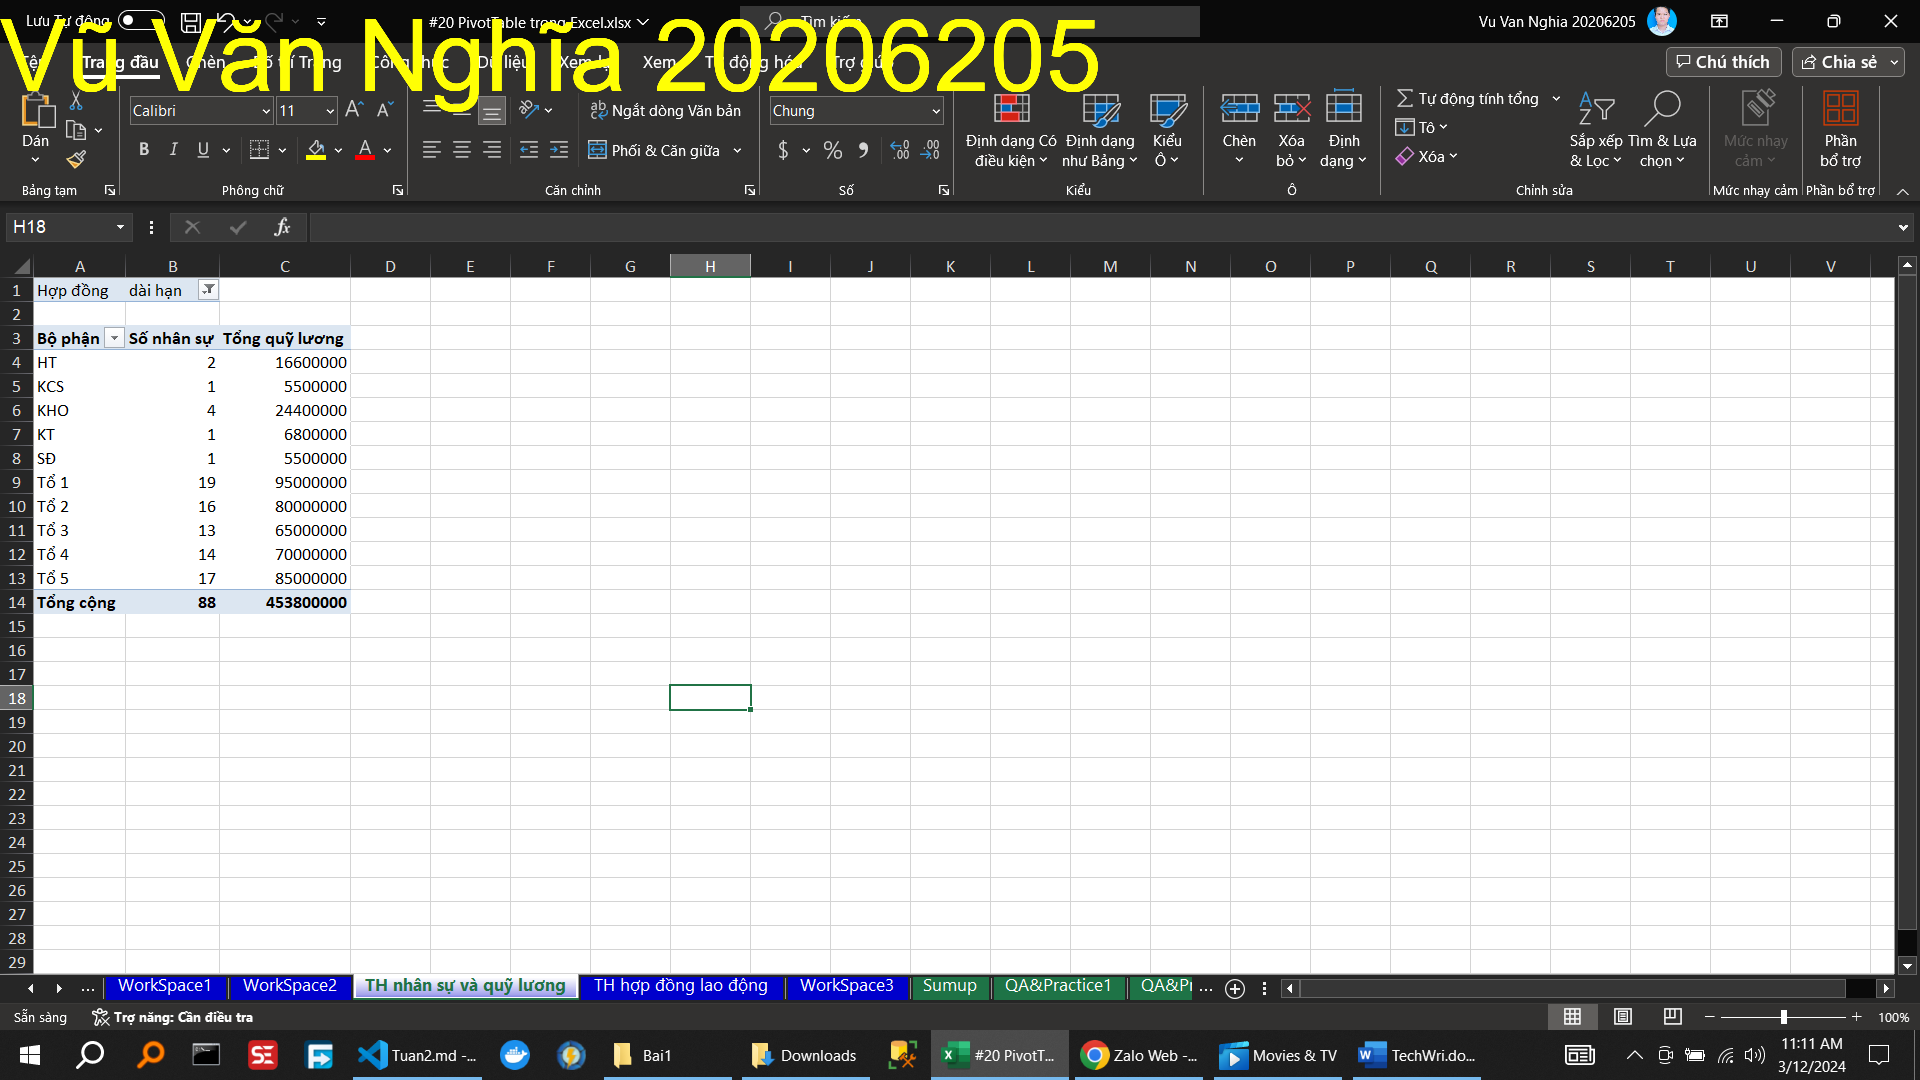
\includegraphics[scale = 0.15]{Bai1/HuongDan/0.png}
\caption{Hướng dẫn tạo báo cáo tổng hợp nhân sự và quỹ lương}
\end{figure}

\begin{figure}[H]
\centering
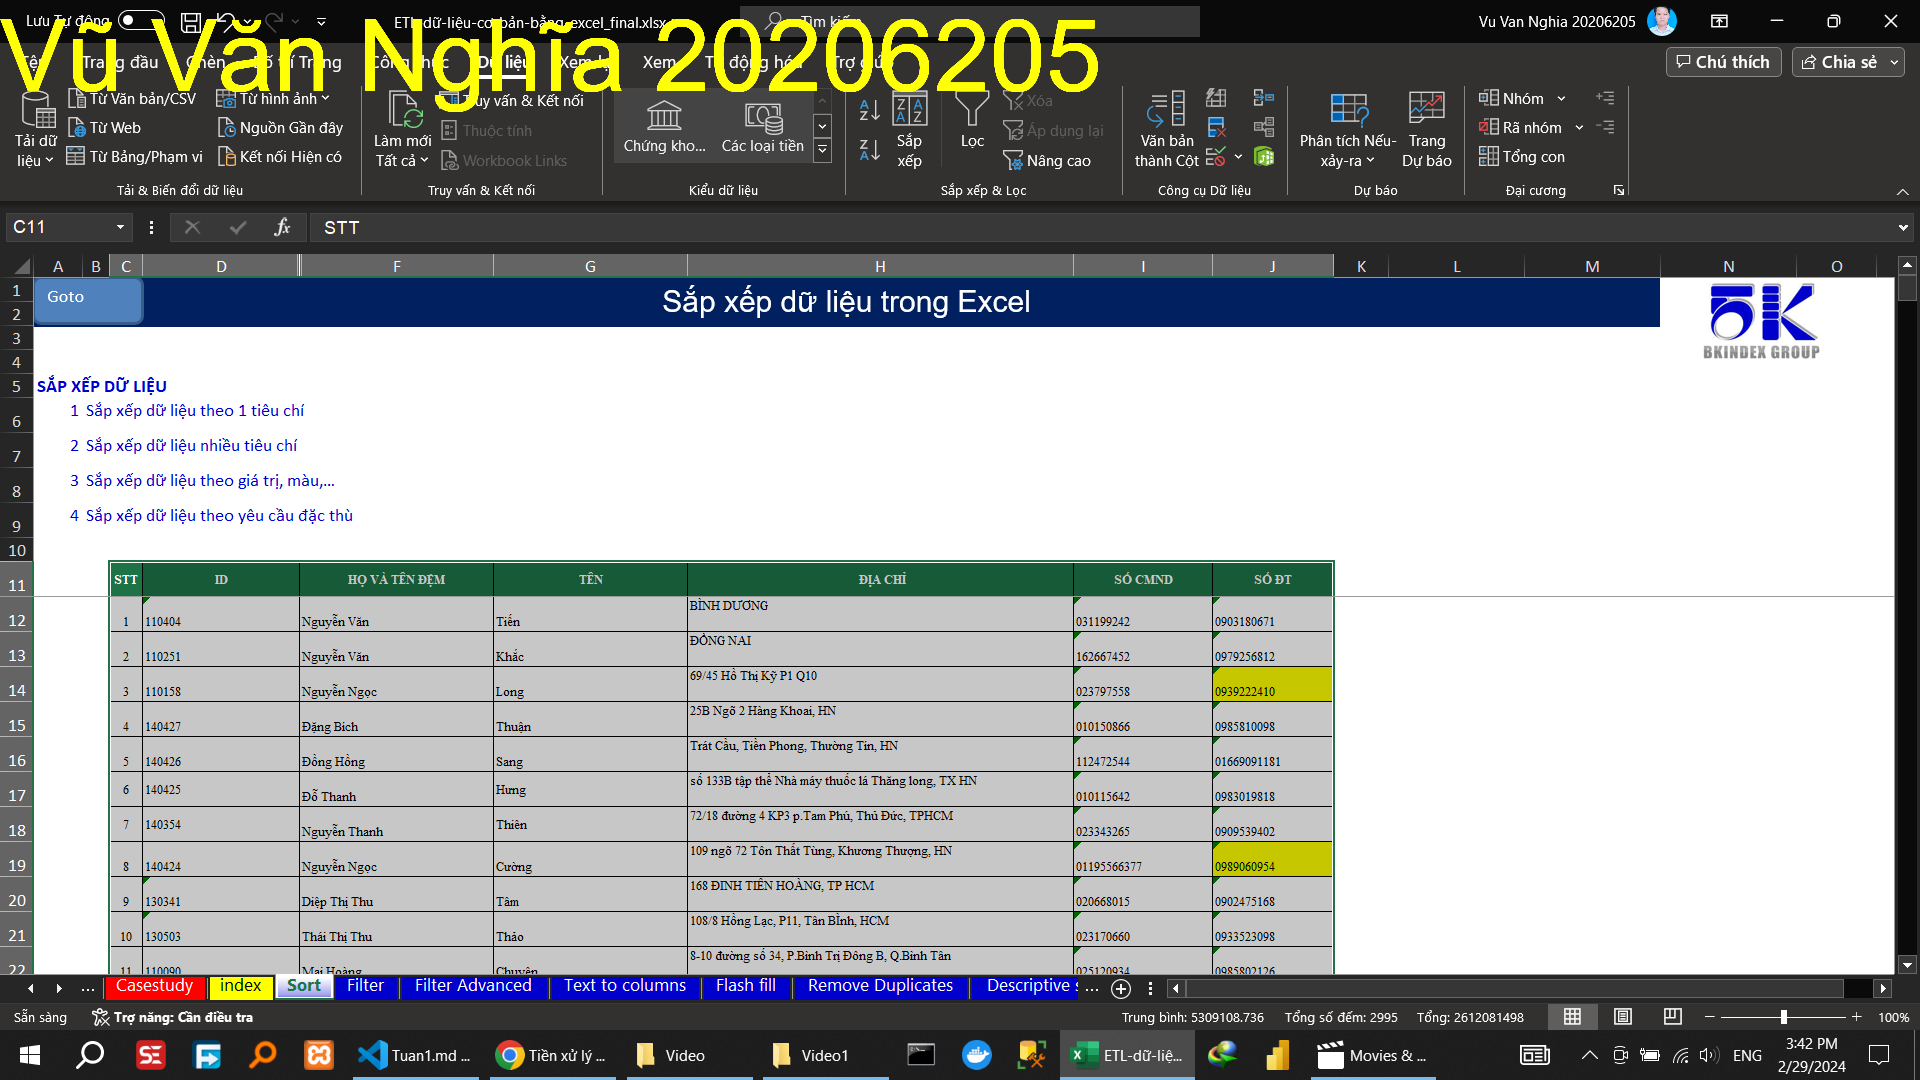
\includegraphics[scale = 0.15]{Bai1/HuongDan/1.png}
\caption{Hướng dẫn tạo báo cáo tổng hợp hợp đồng lao động}
\end{figure}

\begin{figure}[H]
\centering
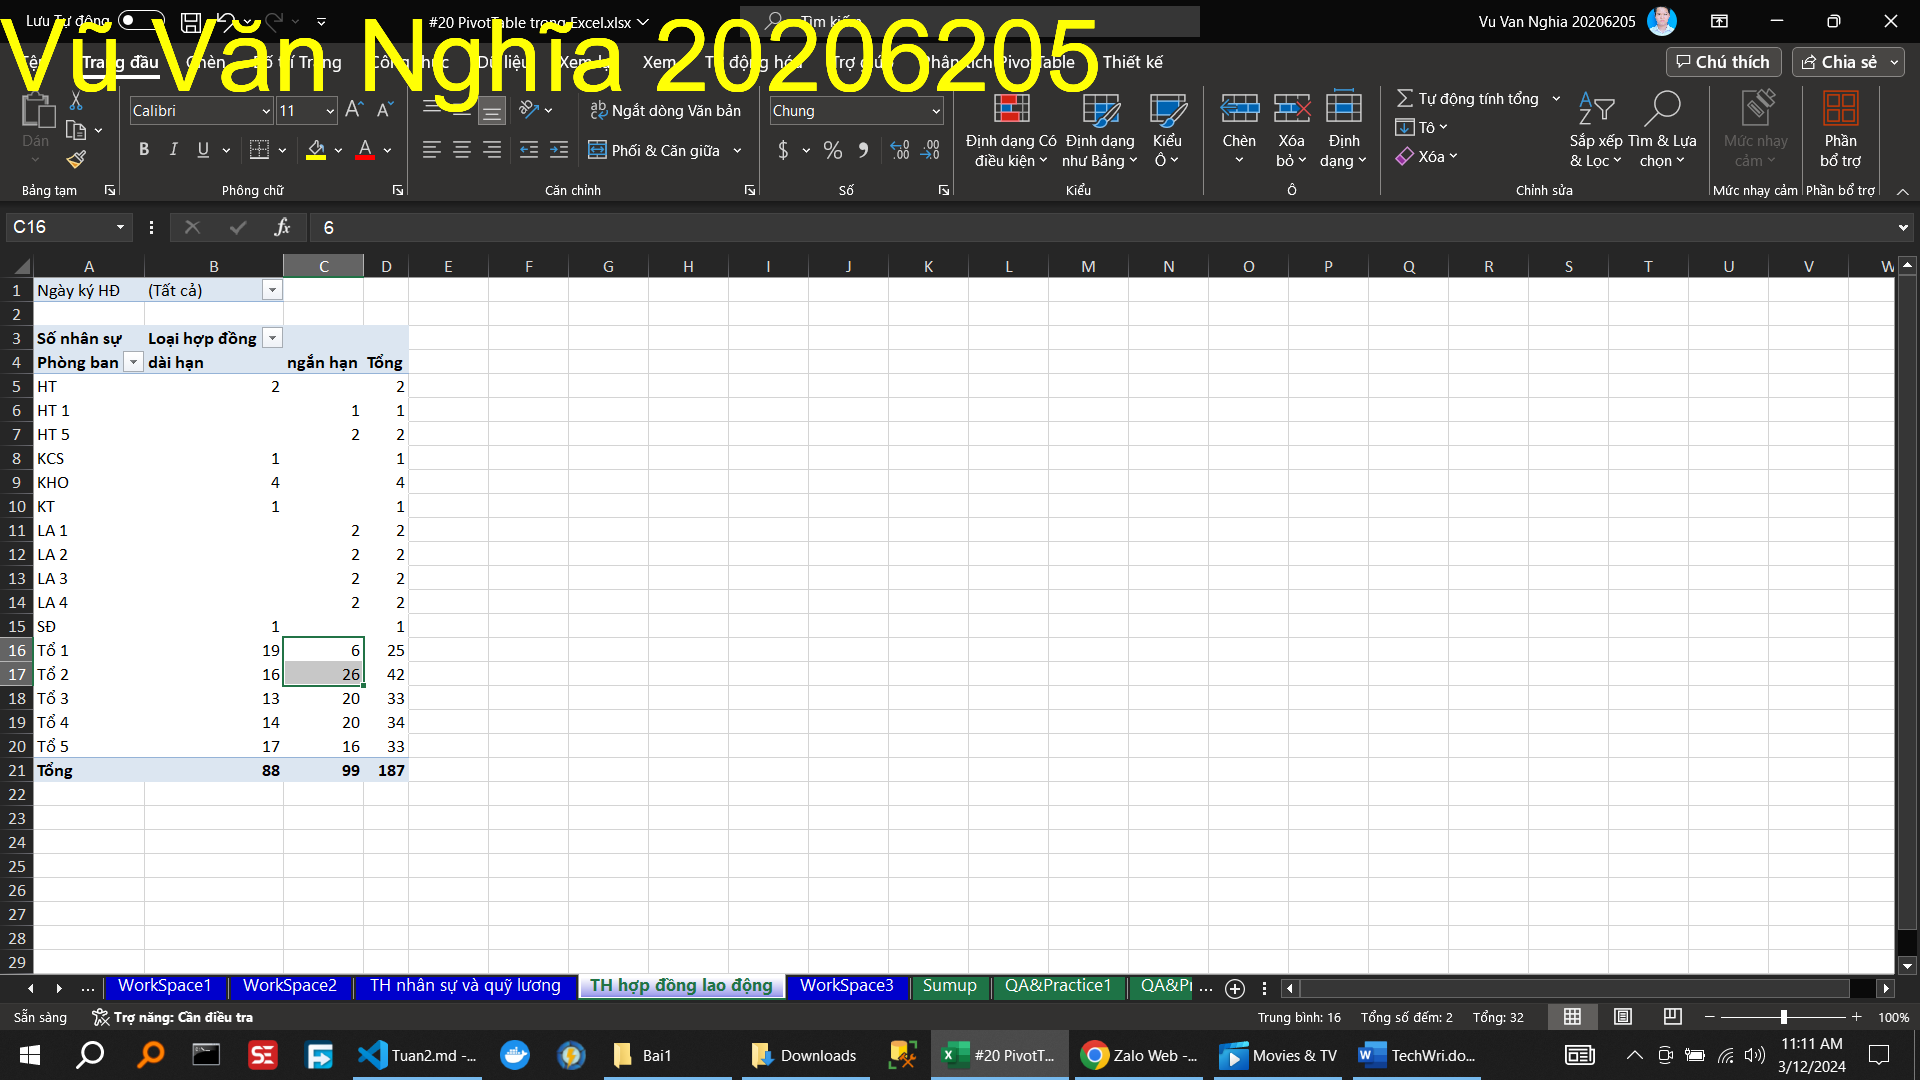
\includegraphics[scale = 0.15]{Bai1/HuongDan/2.png}
\caption{Hướng dẫn làm mới dữ liệu báo cáo}
\end{figure}

\begin{figure}[H]
\centering
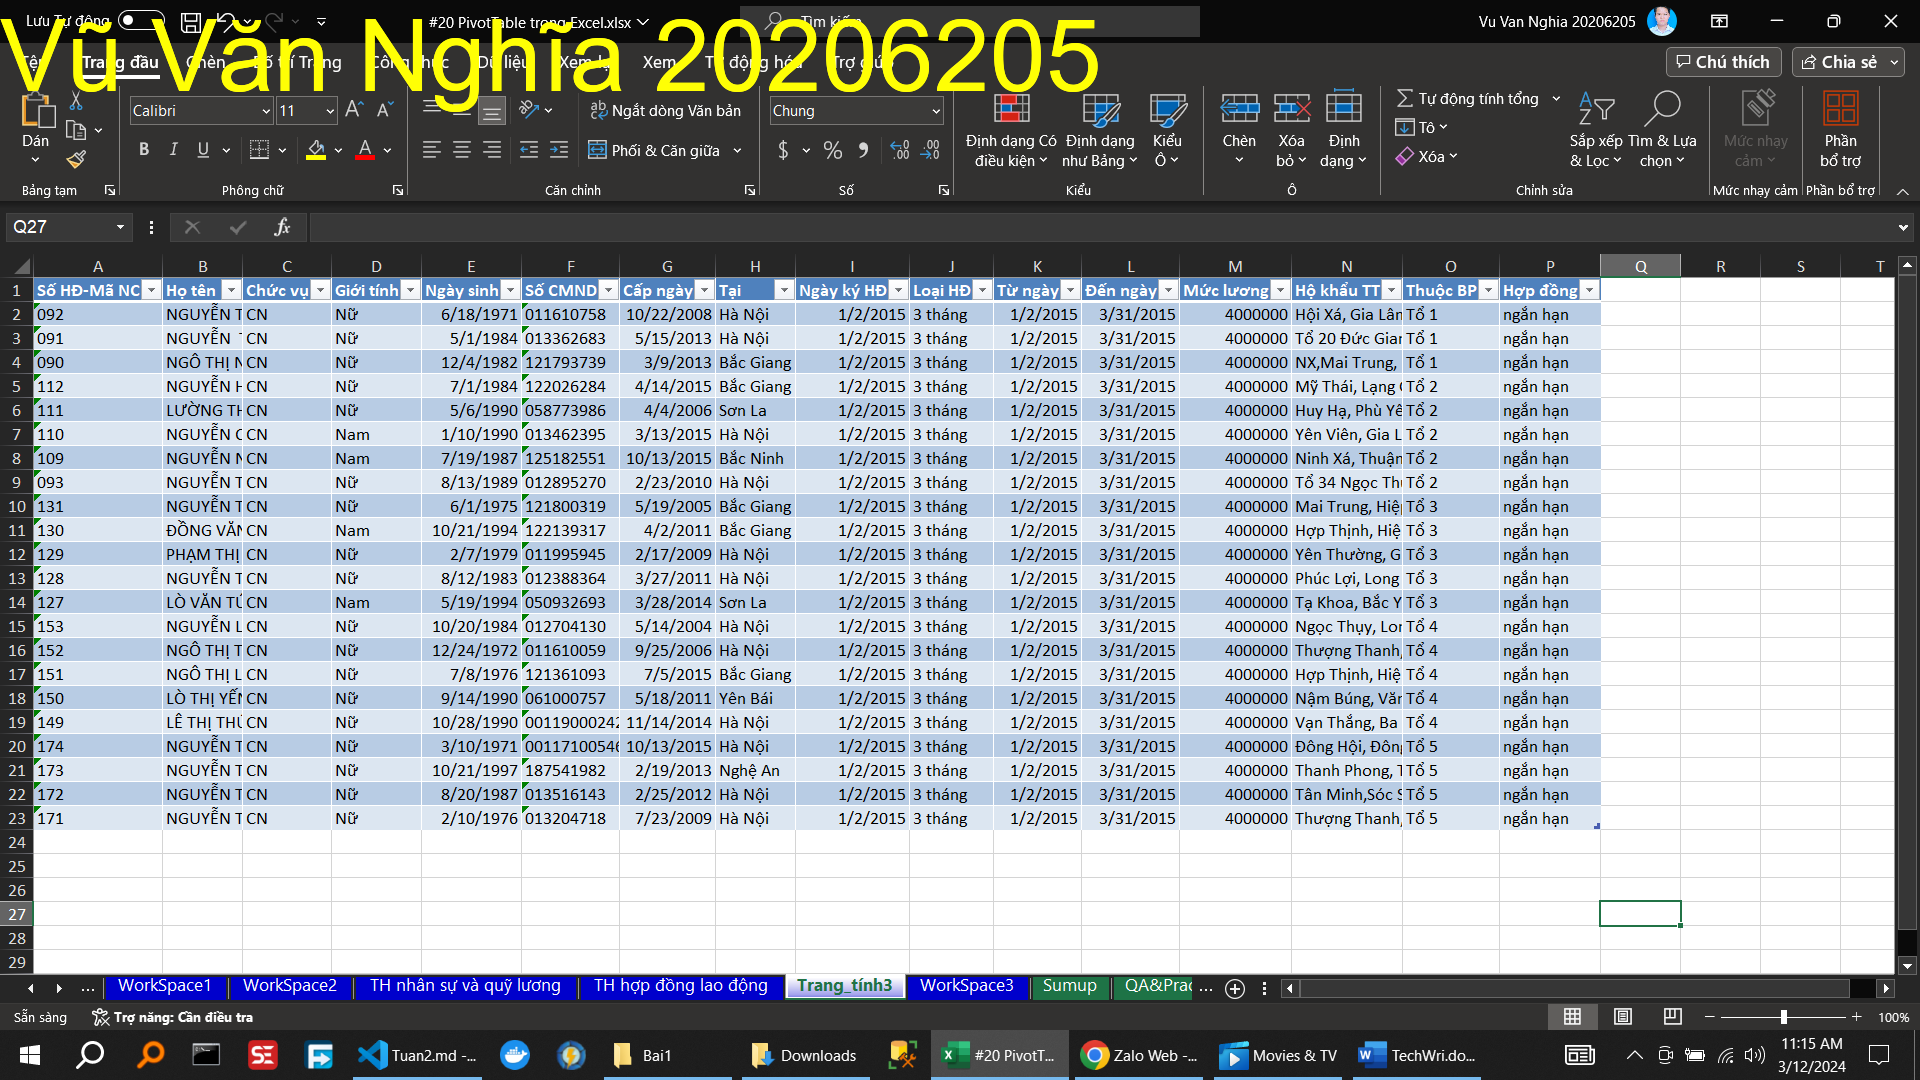
\includegraphics[scale = 0.15]{Bai1/HuongDan/3.png}
\caption{Hướng dẫn lấy dữ liệu chi tiết từ báo cáo}
\end{figure}

\begin{figure}[H]
\centering
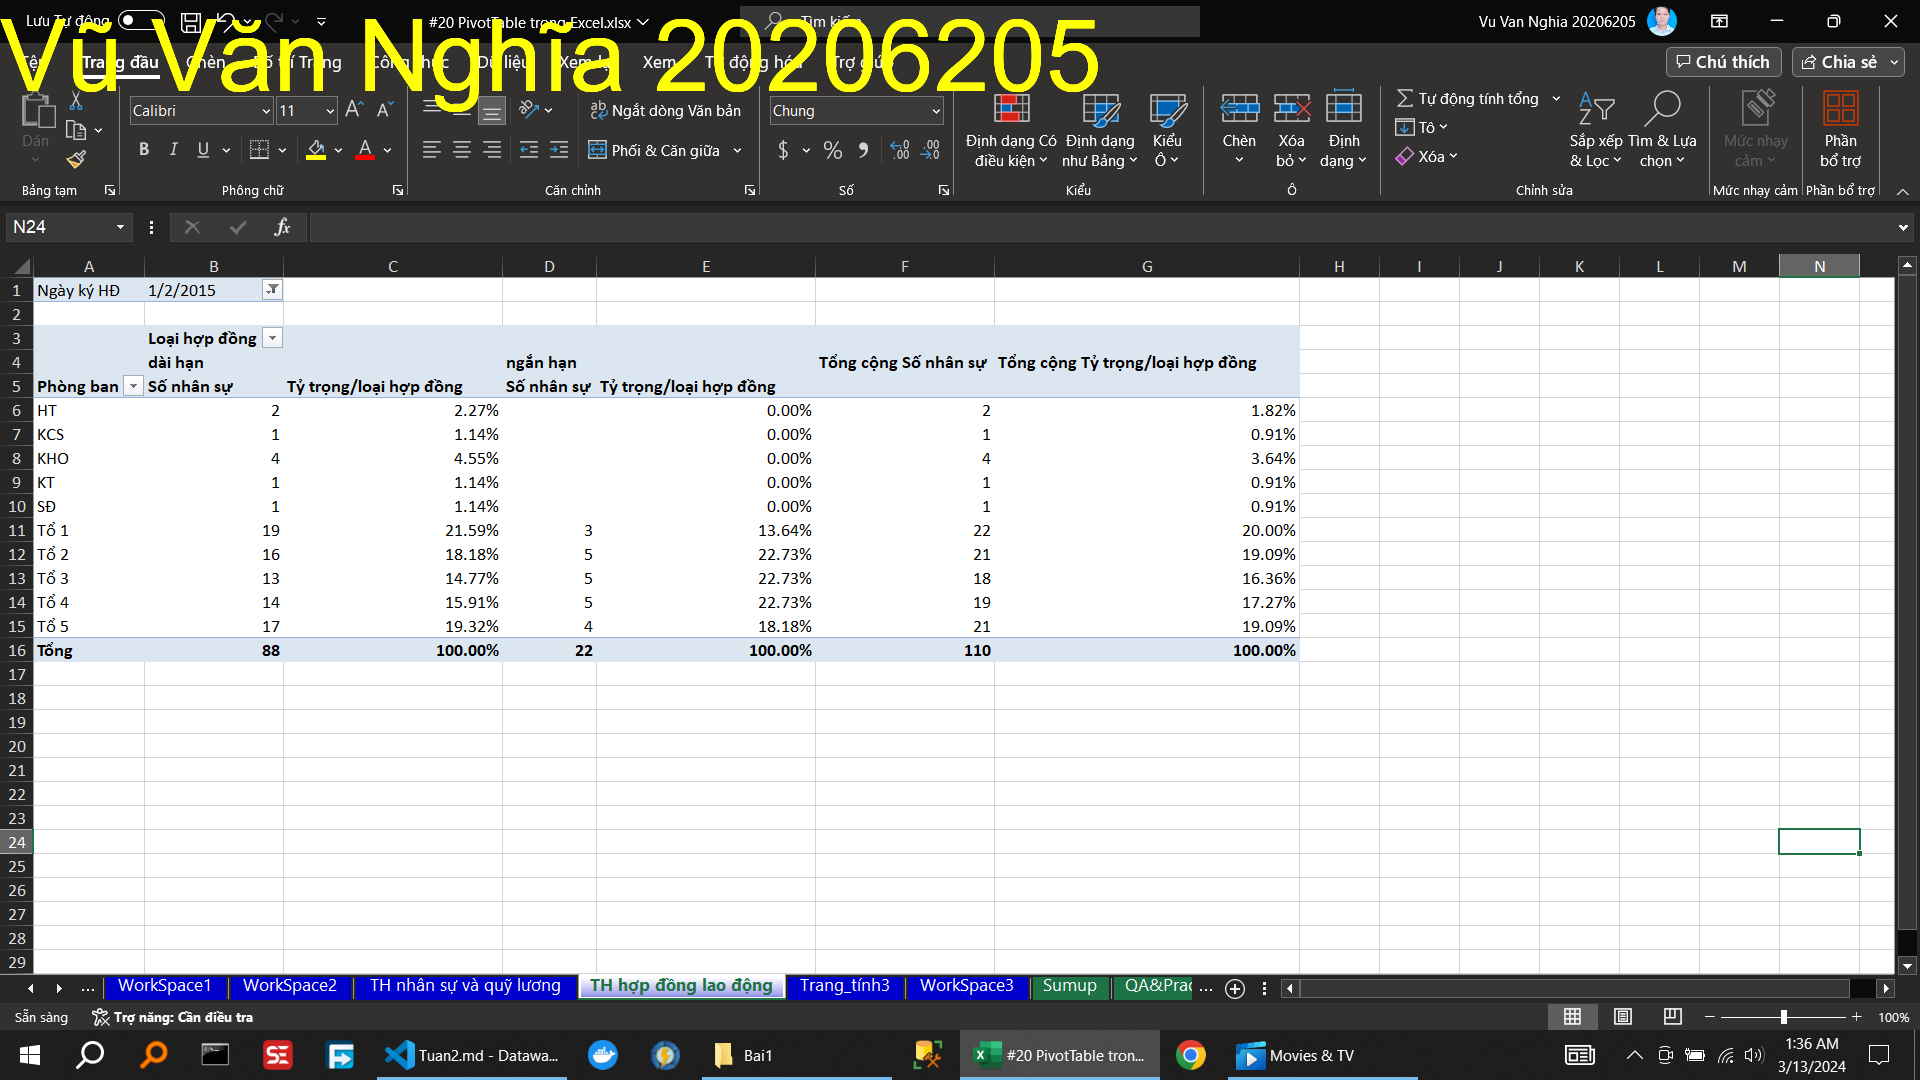
\includegraphics[scale = 0.15]{Bai1/HuongDan/4.png}
\caption{Hướng dẫn định dạng dữ liệu trên báo cáo}
\end{figure}

\begin{figure}[H]
\centering
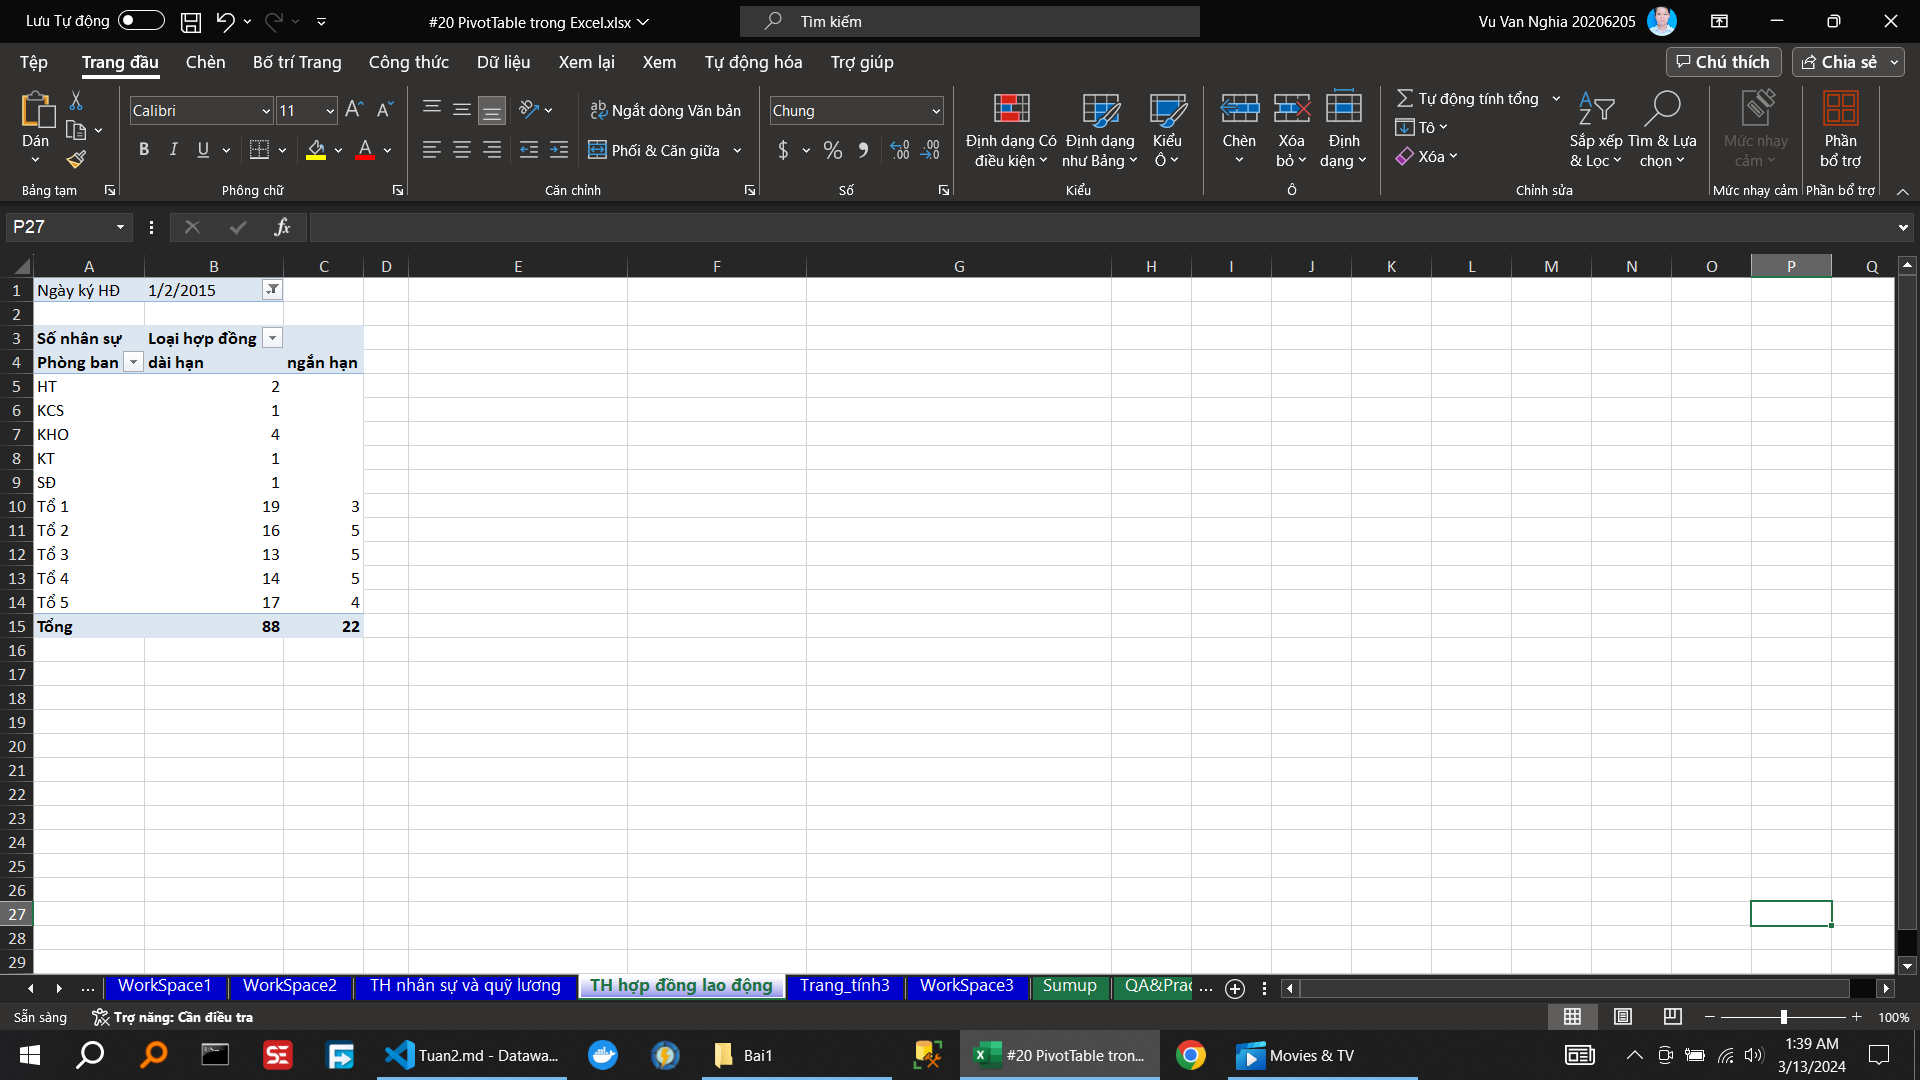
\includegraphics[scale = 0.15]{Bai1/HuongDan/5.png}
\caption{Hướng dẫn thêm các cột/dòng tổng hợp}
\end{figure}

\begin{figure}[H]
\centering
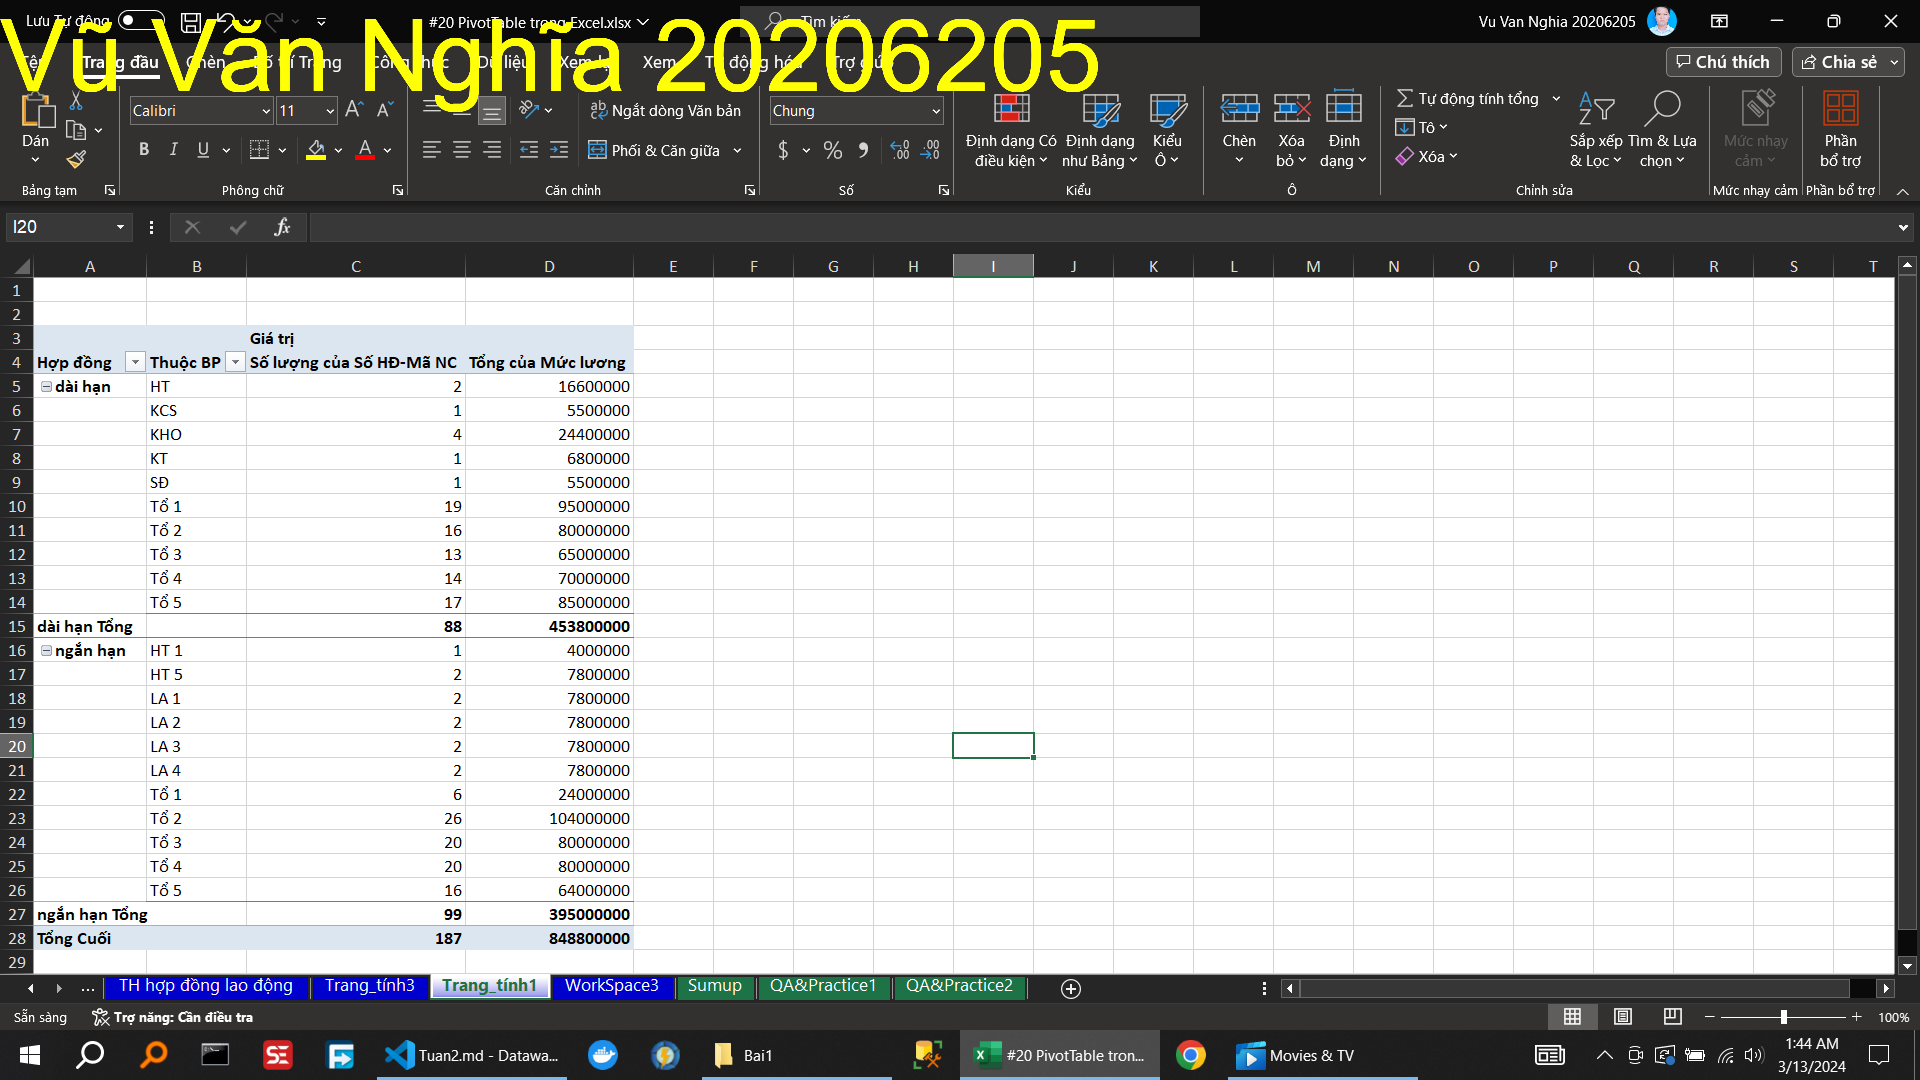
\includegraphics[scale = 0.15]{Bai1/HuongDan/6.png}
\caption{Hướng dẫn tùy chỉnh báo cáo dạng cổ điển}
\end{figure}

\begin{figure}[H]
\centering
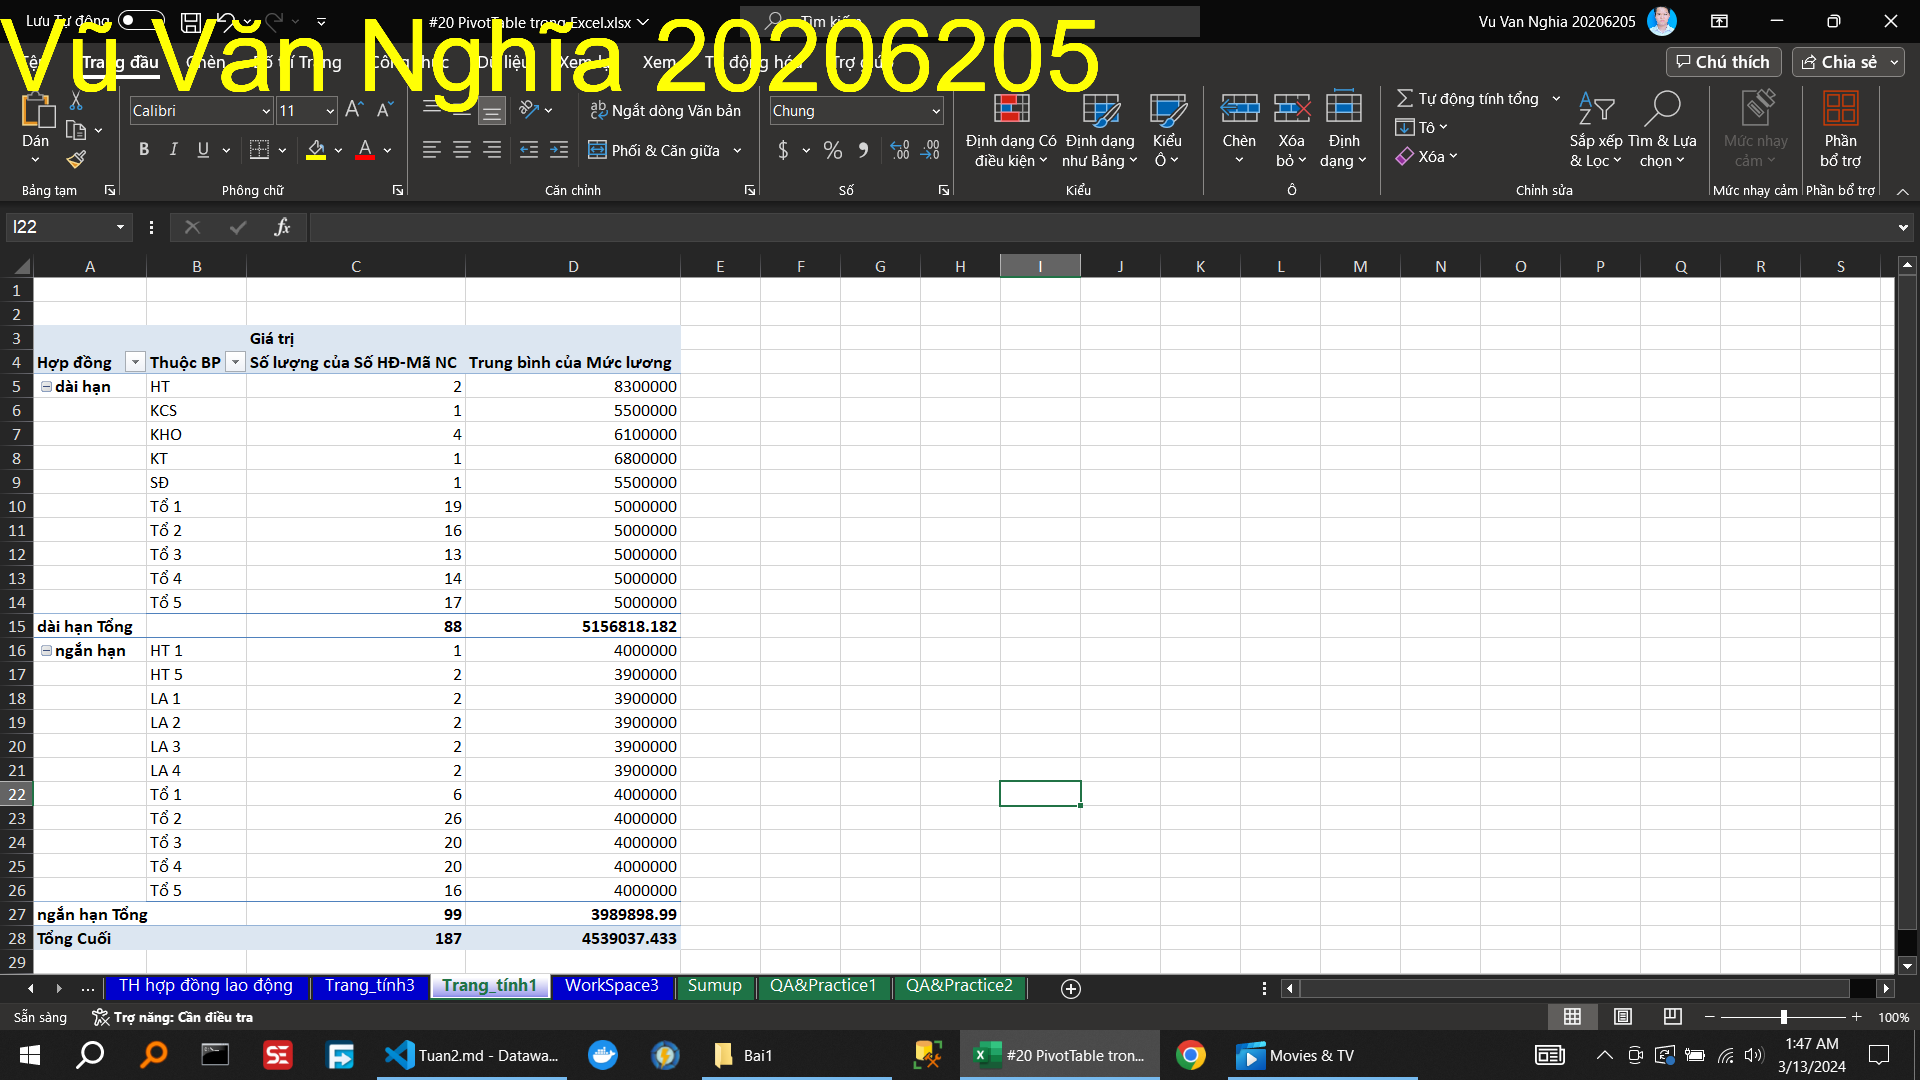
\includegraphics[scale = 0.15]{Bai1/HuongDan/7.png}
\caption{Hướng dẫn tùy chỉnh công thức tính}
\end{figure}

\begin{figure}[H]
\centering
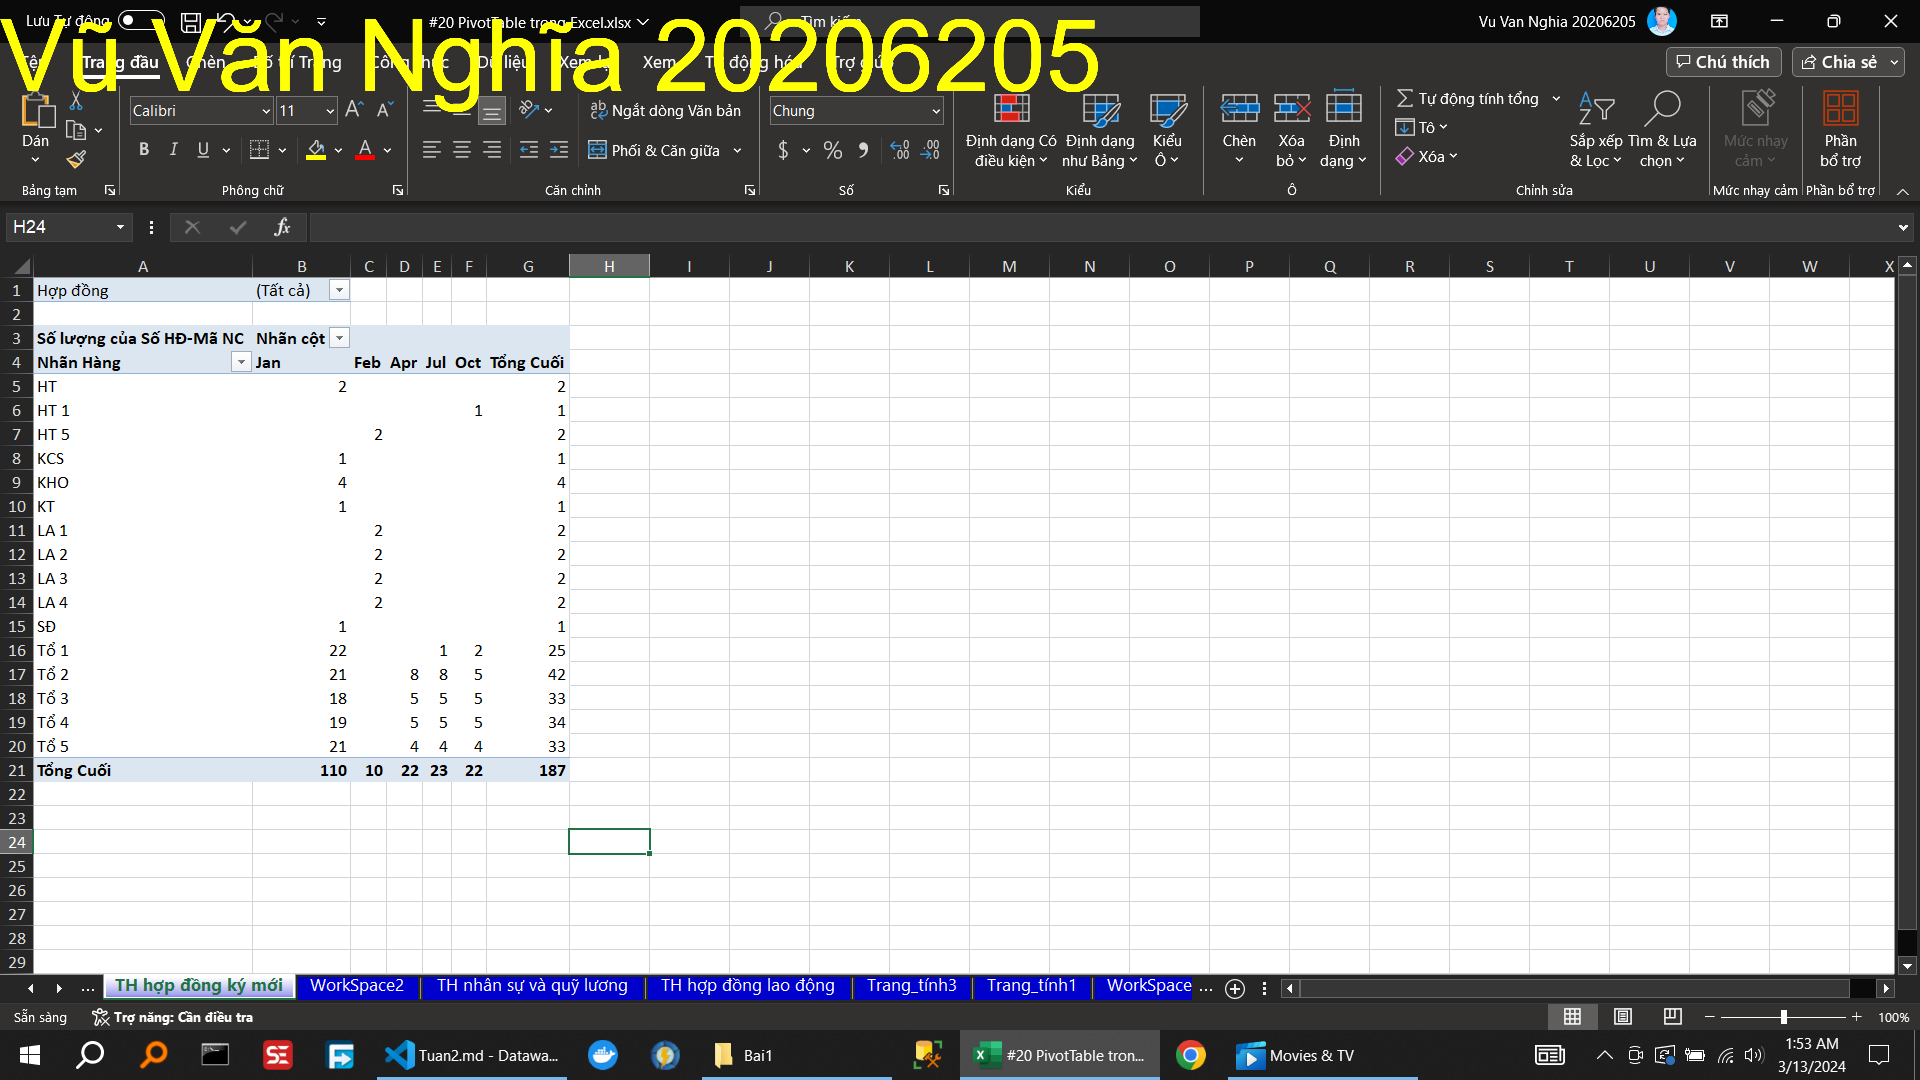
\includegraphics[scale = 0.15]{Bai1/HuongDan/8.png}
\caption{Hướng dẫn nhóm các loại dữ liệu (dạng ngày tháng)}
\end{figure}

\begin{figure}[H]
\centering
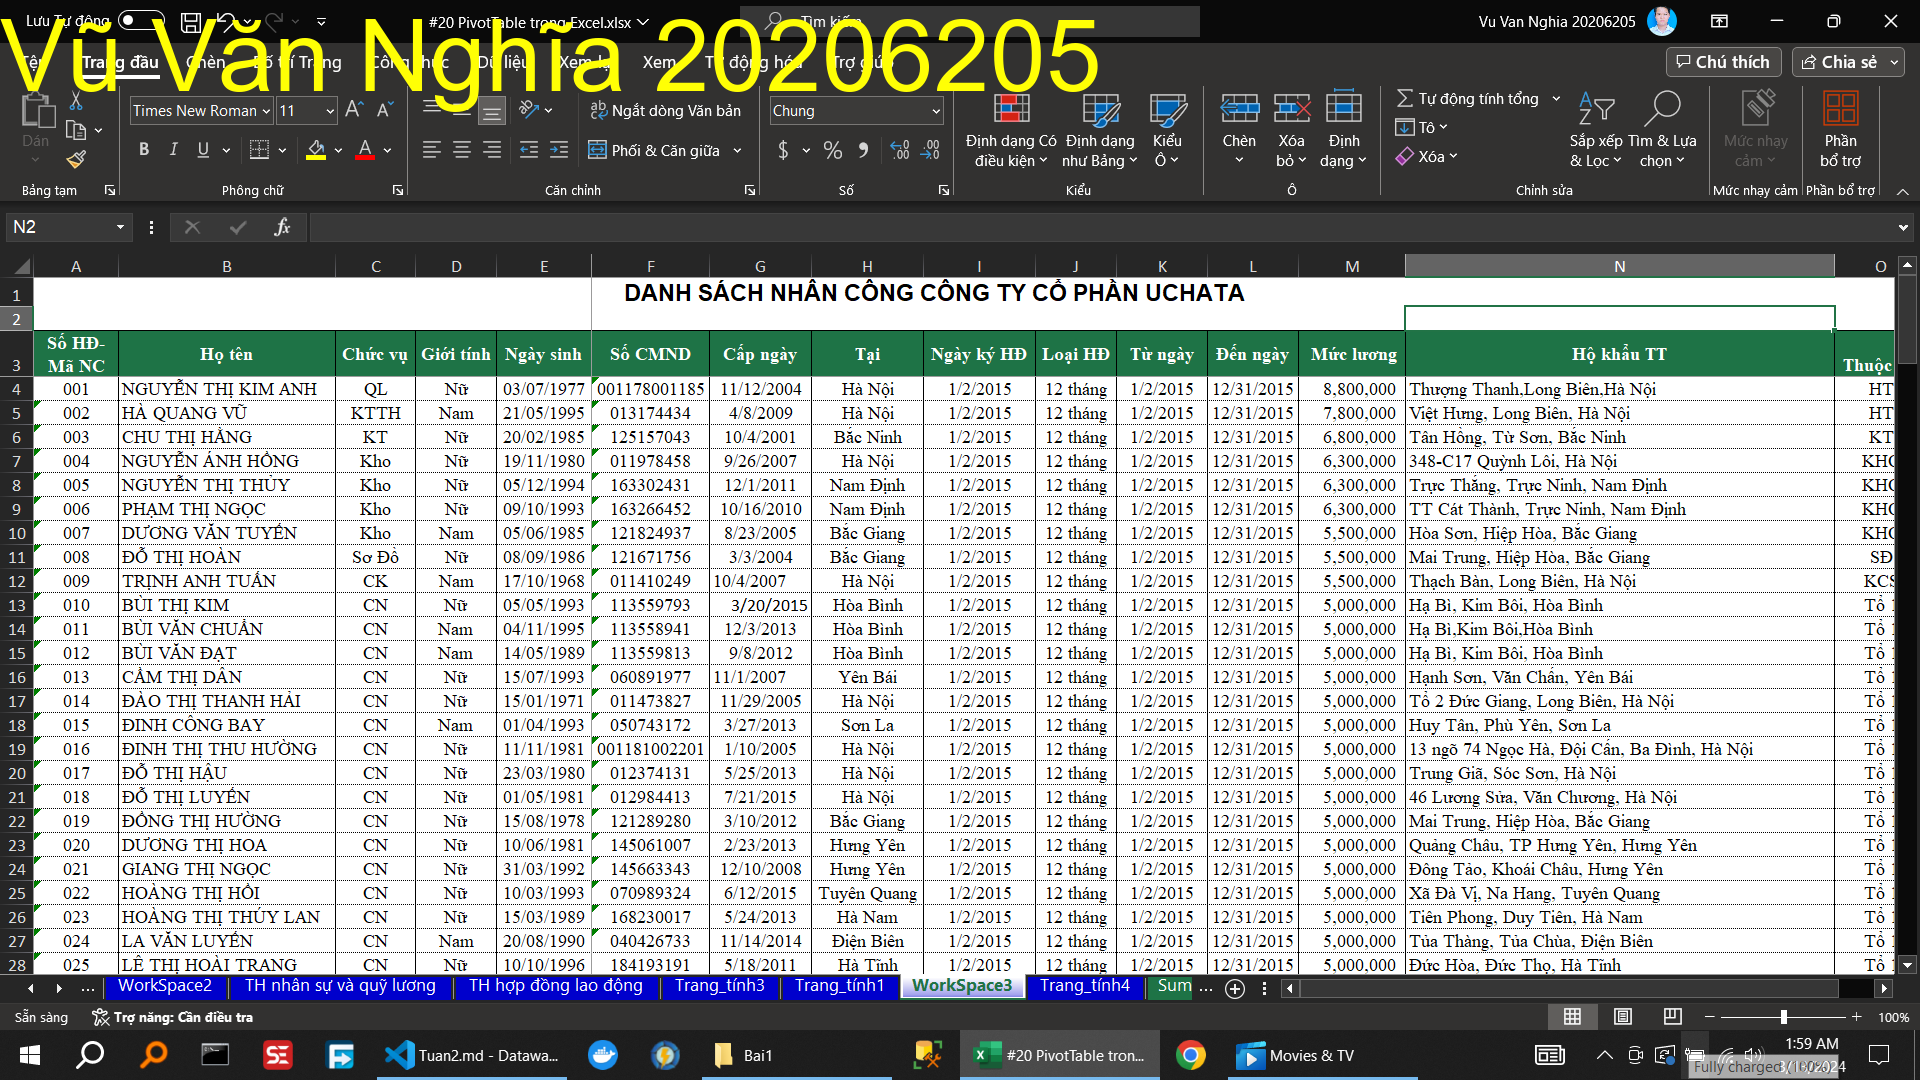
\includegraphics[scale = 0.15]{Bai1/HuongDan/9.png}
\caption{Hướng dẫn tiền xử lý dữ liệu}
\end{figure}

\begin{figure}[H]
\centering
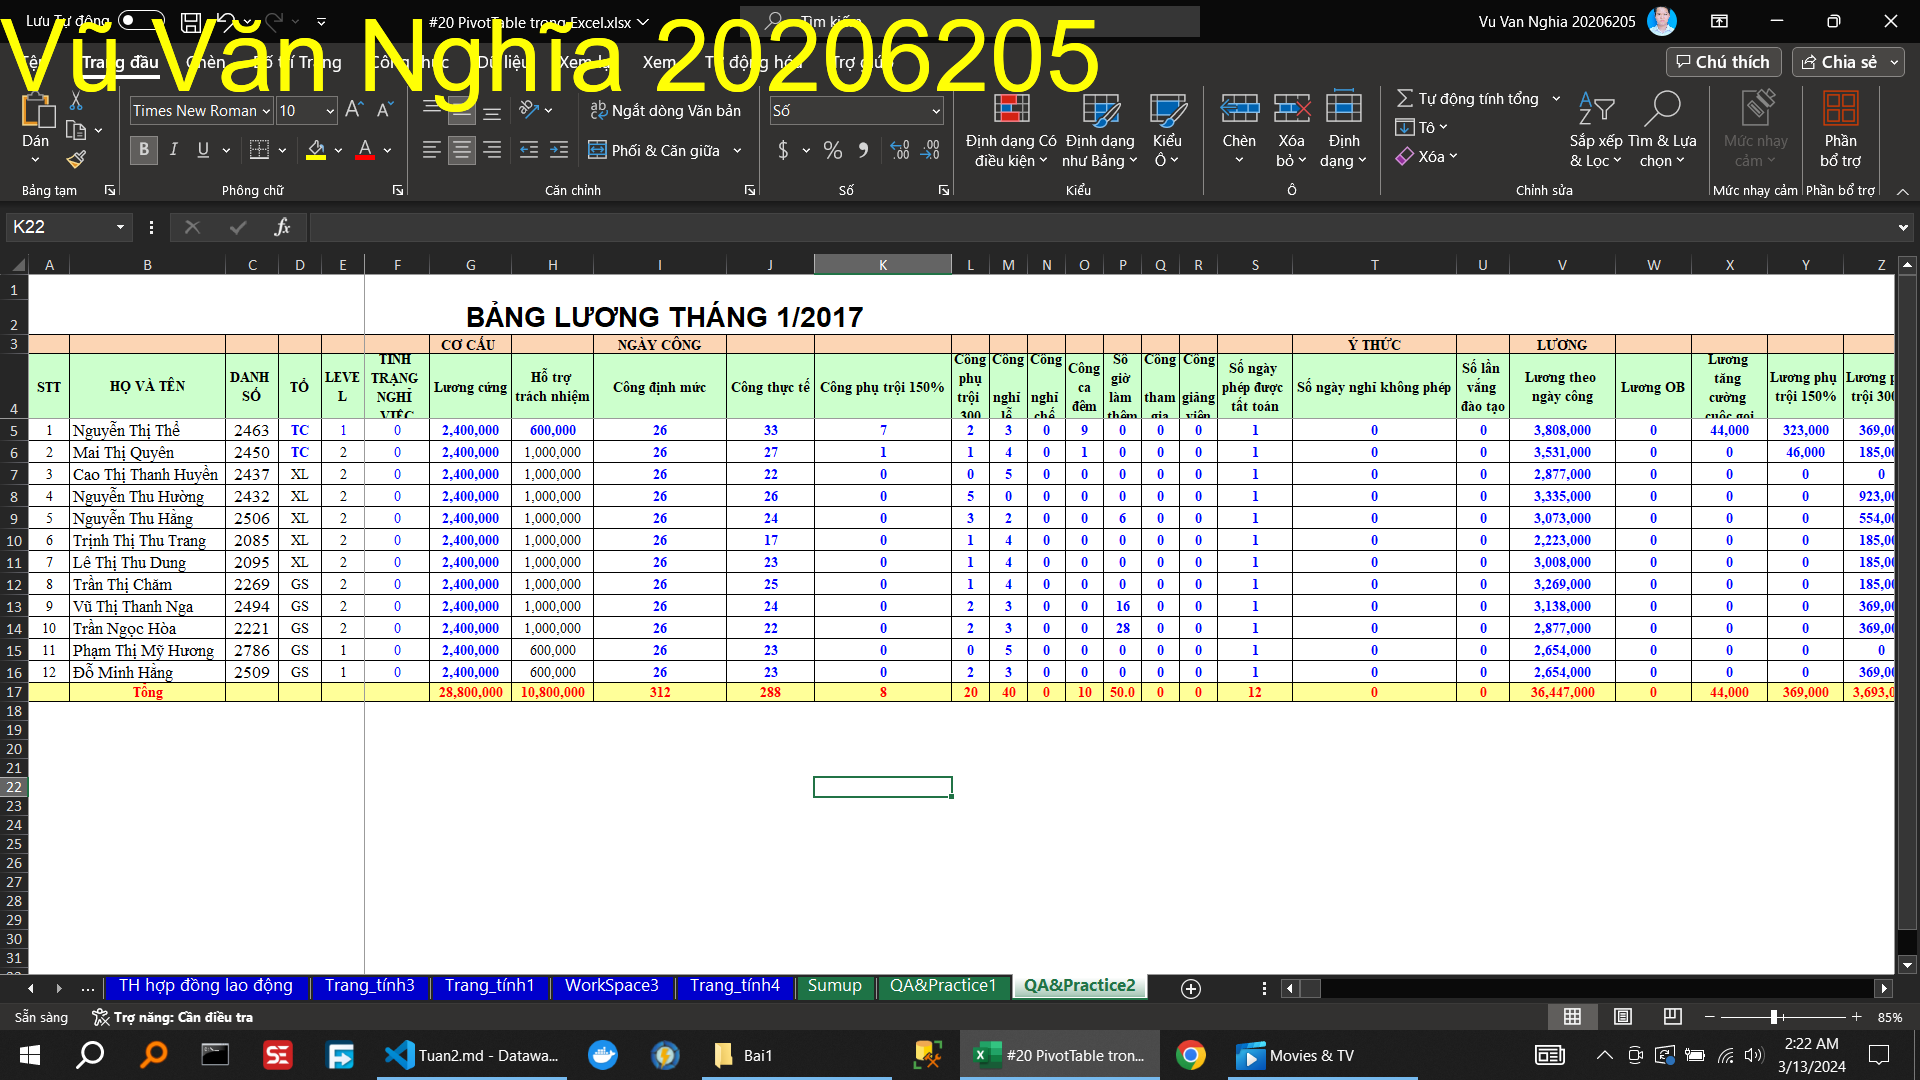
\includegraphics[scale = 0.15]{Bai1/ThucHanh/0.png}
\caption{Thực hành tiền xử lý dữ liệu}
\end{figure}

\begin{figure}[H]
\centering
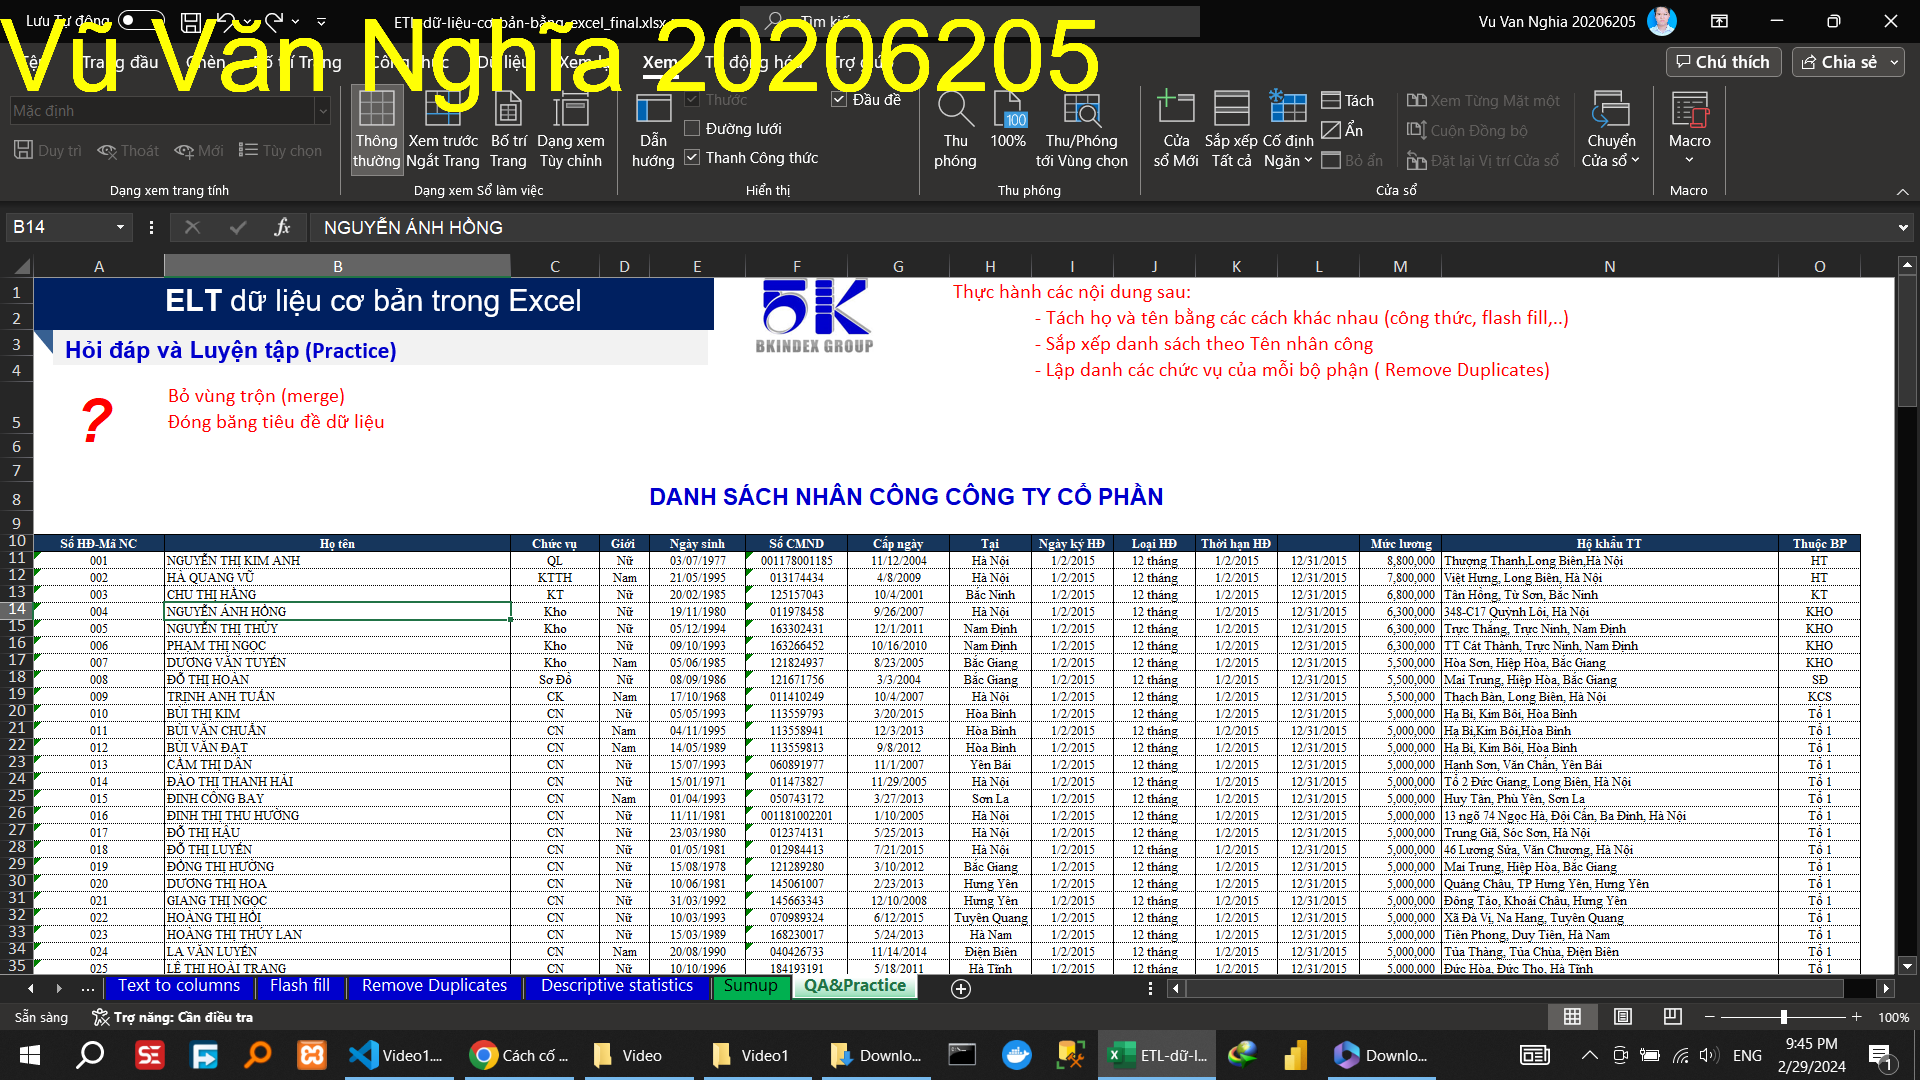
\includegraphics[scale = 0.15]{Bai1/ThucHanh/1.png}
\caption{Thực hành tạo báo cáo tổng hợp}
\end{figure}

\begin{figure}[H]
\centering
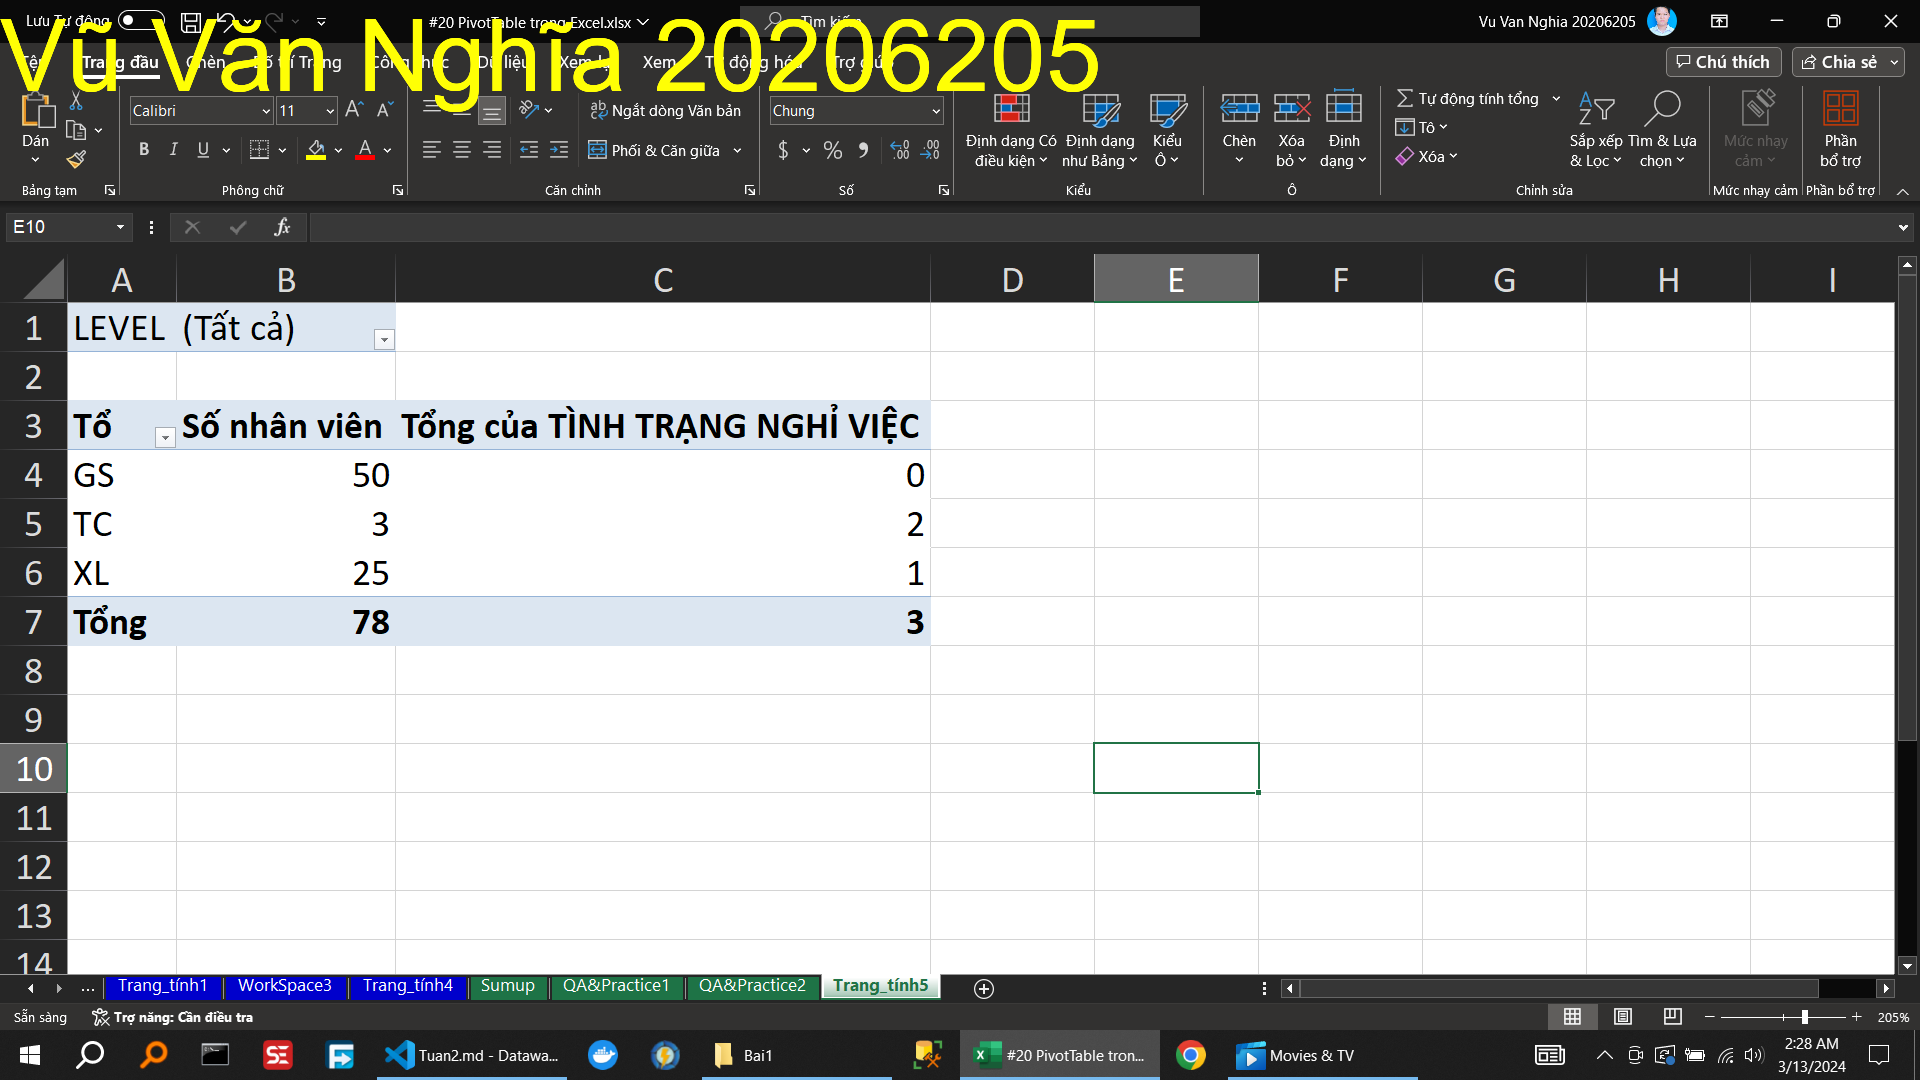
\includegraphics[scale = 0.15]{Bai1/ThucHanh/2.png}
\caption{Thực hành làm mới dữ liệu báo cáo}
\end{figure}

%%%%%%%%%%%%%%%%%%%%%%%%%%%%%%%%%%%%%%%%%%%%%%%%%%%%%%%
\subsection{Bài 2}

\begin{figure}[H]
\centering
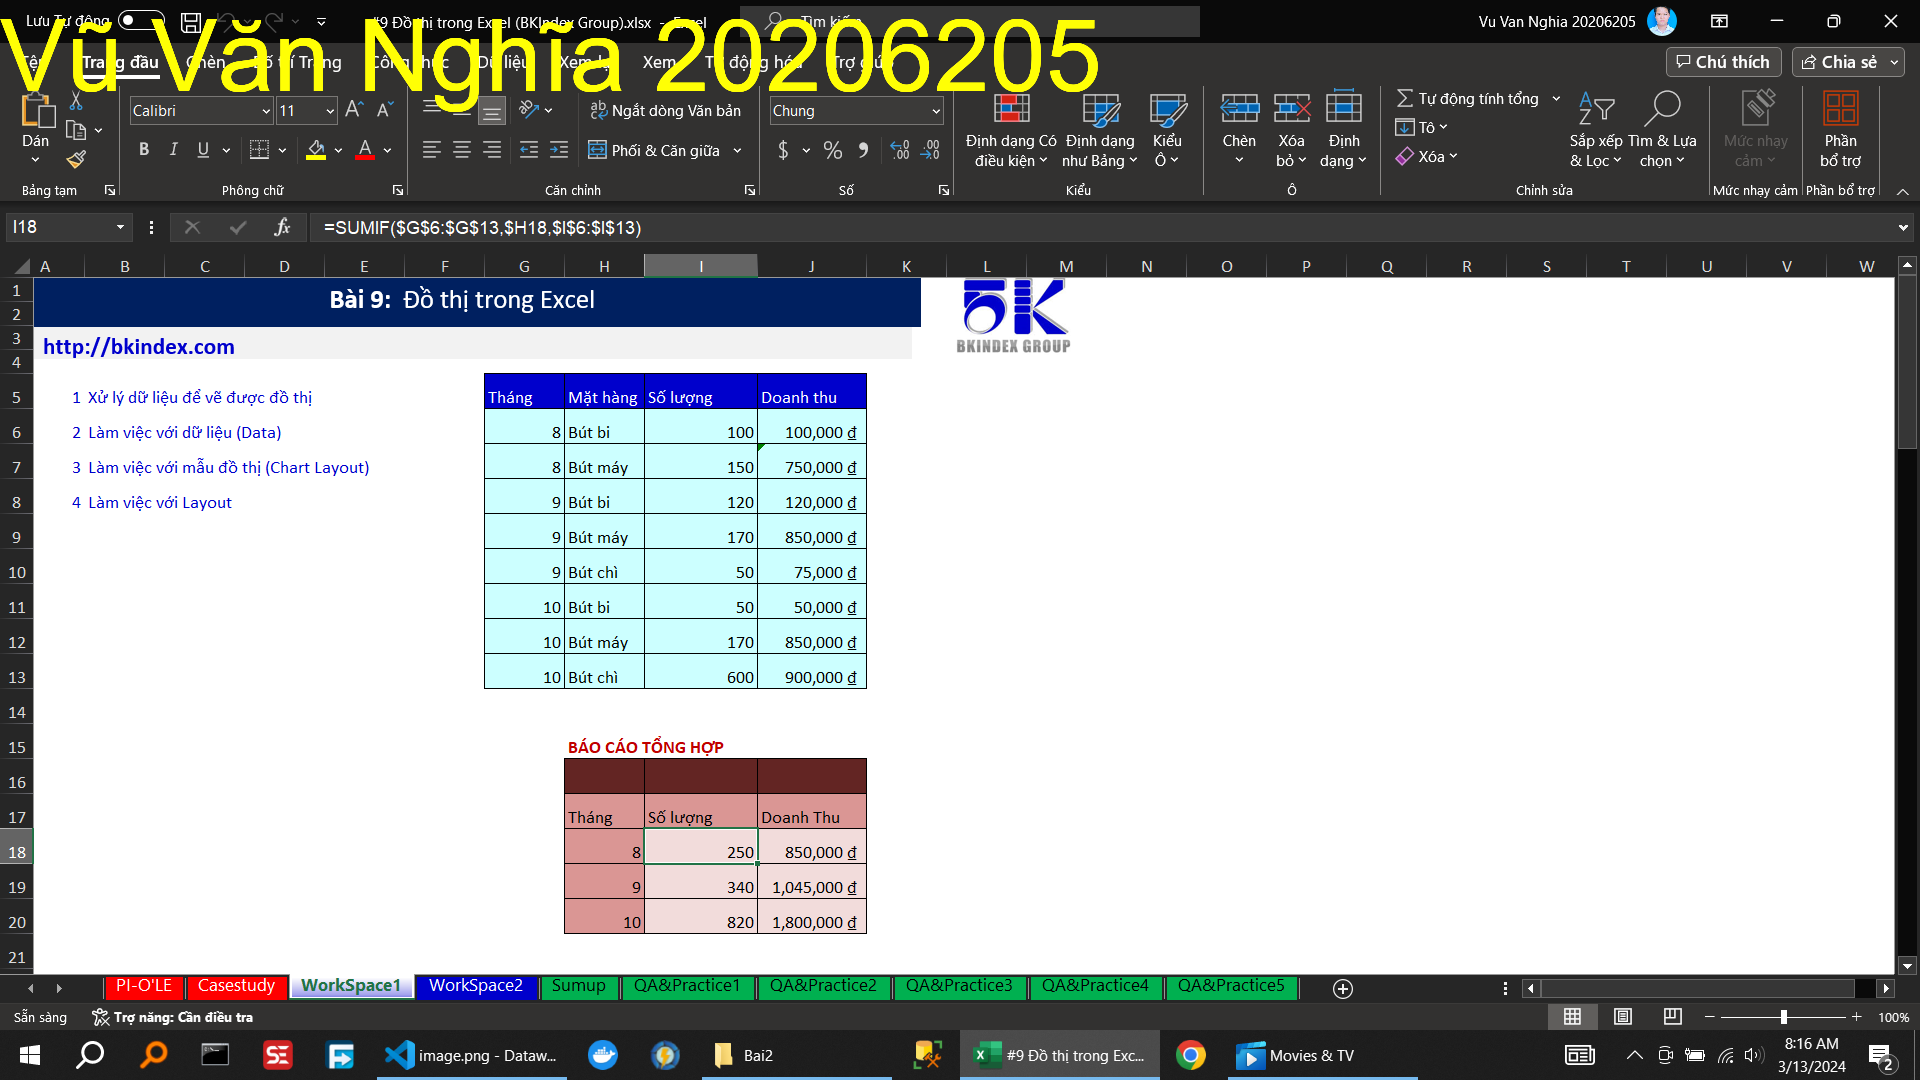
\includegraphics[scale = 0.15]{Bai2/HuongDan/0.png}
\caption{Hướng dẫn xử lý dữ liệu để vẽ được đồ thị}
\end{figure}

\begin{figure}[H]
\centering
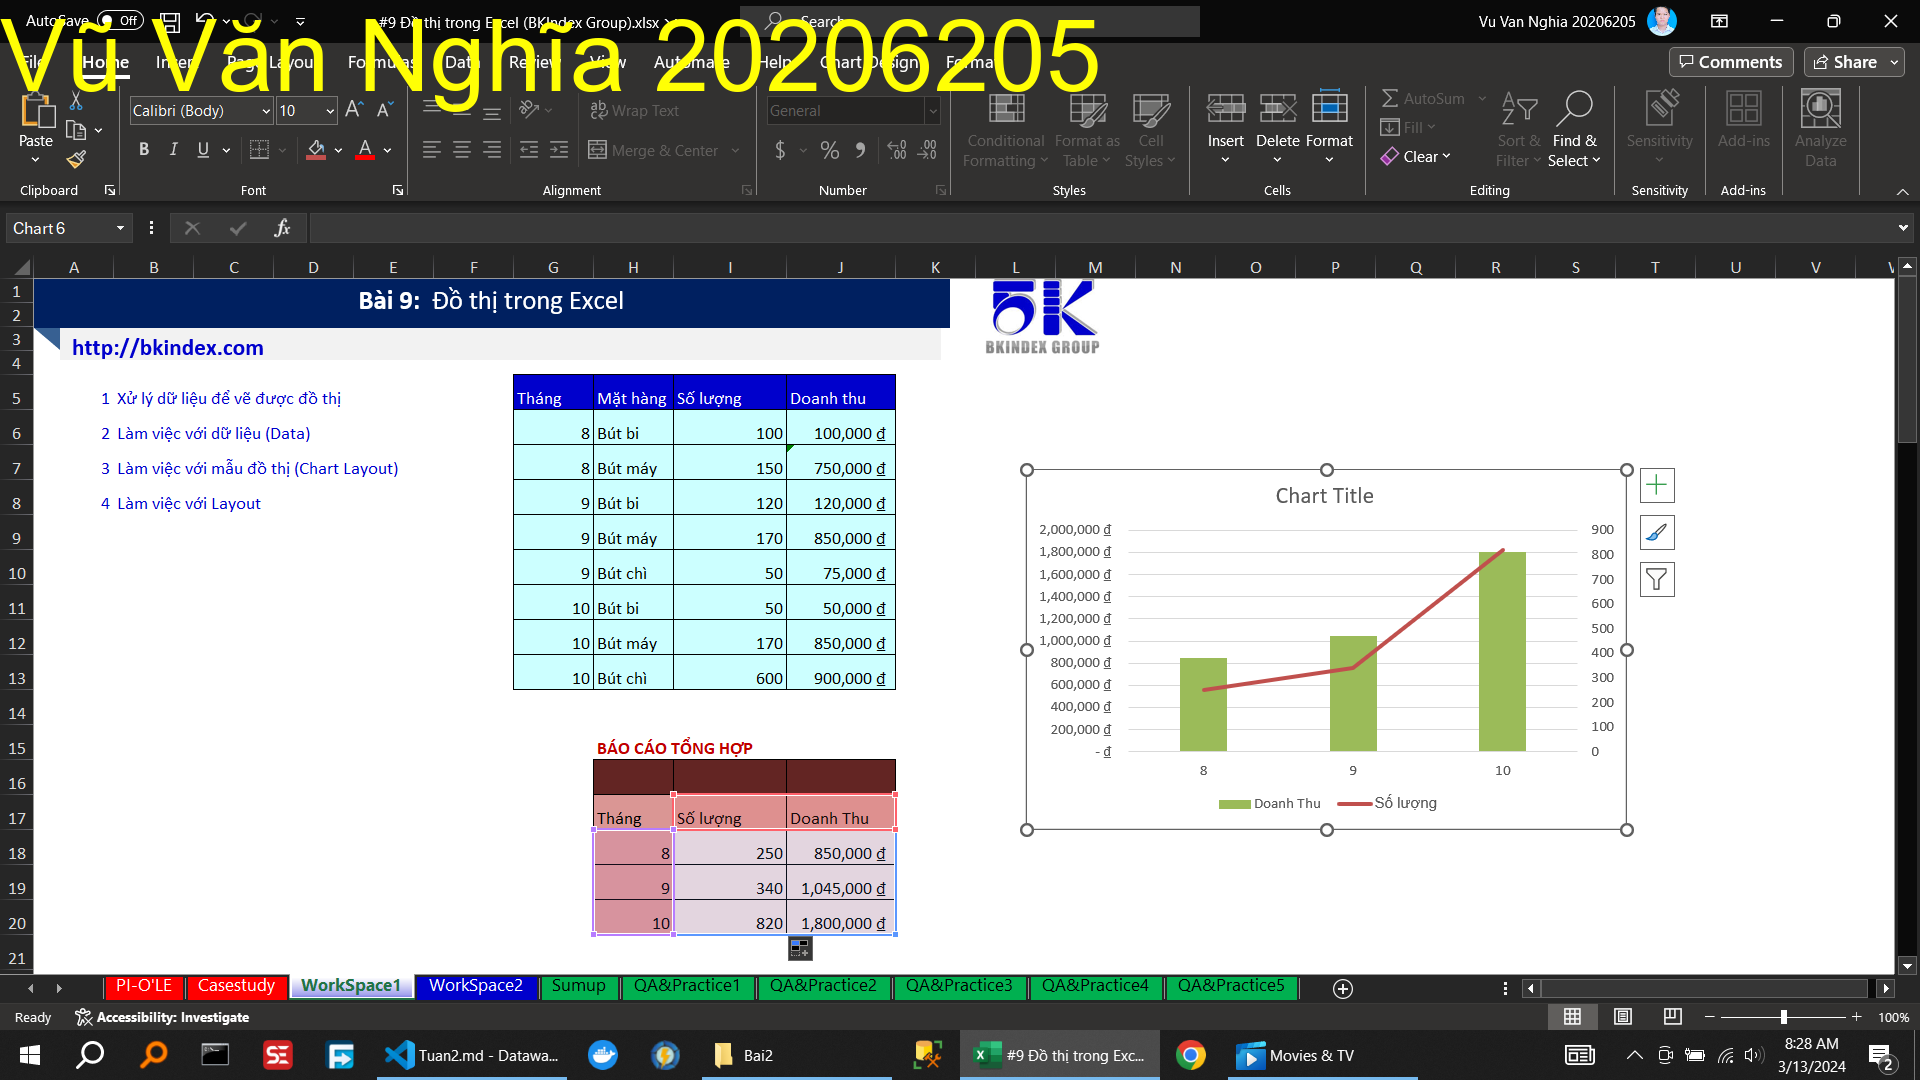
\includegraphics[scale = 0.15]{Bai2/HuongDan/1.png}
\caption{Hướng dẫn vẽ được đồ thị với dữ liệu}
\end{figure}

\begin{figure}[H]
\centering
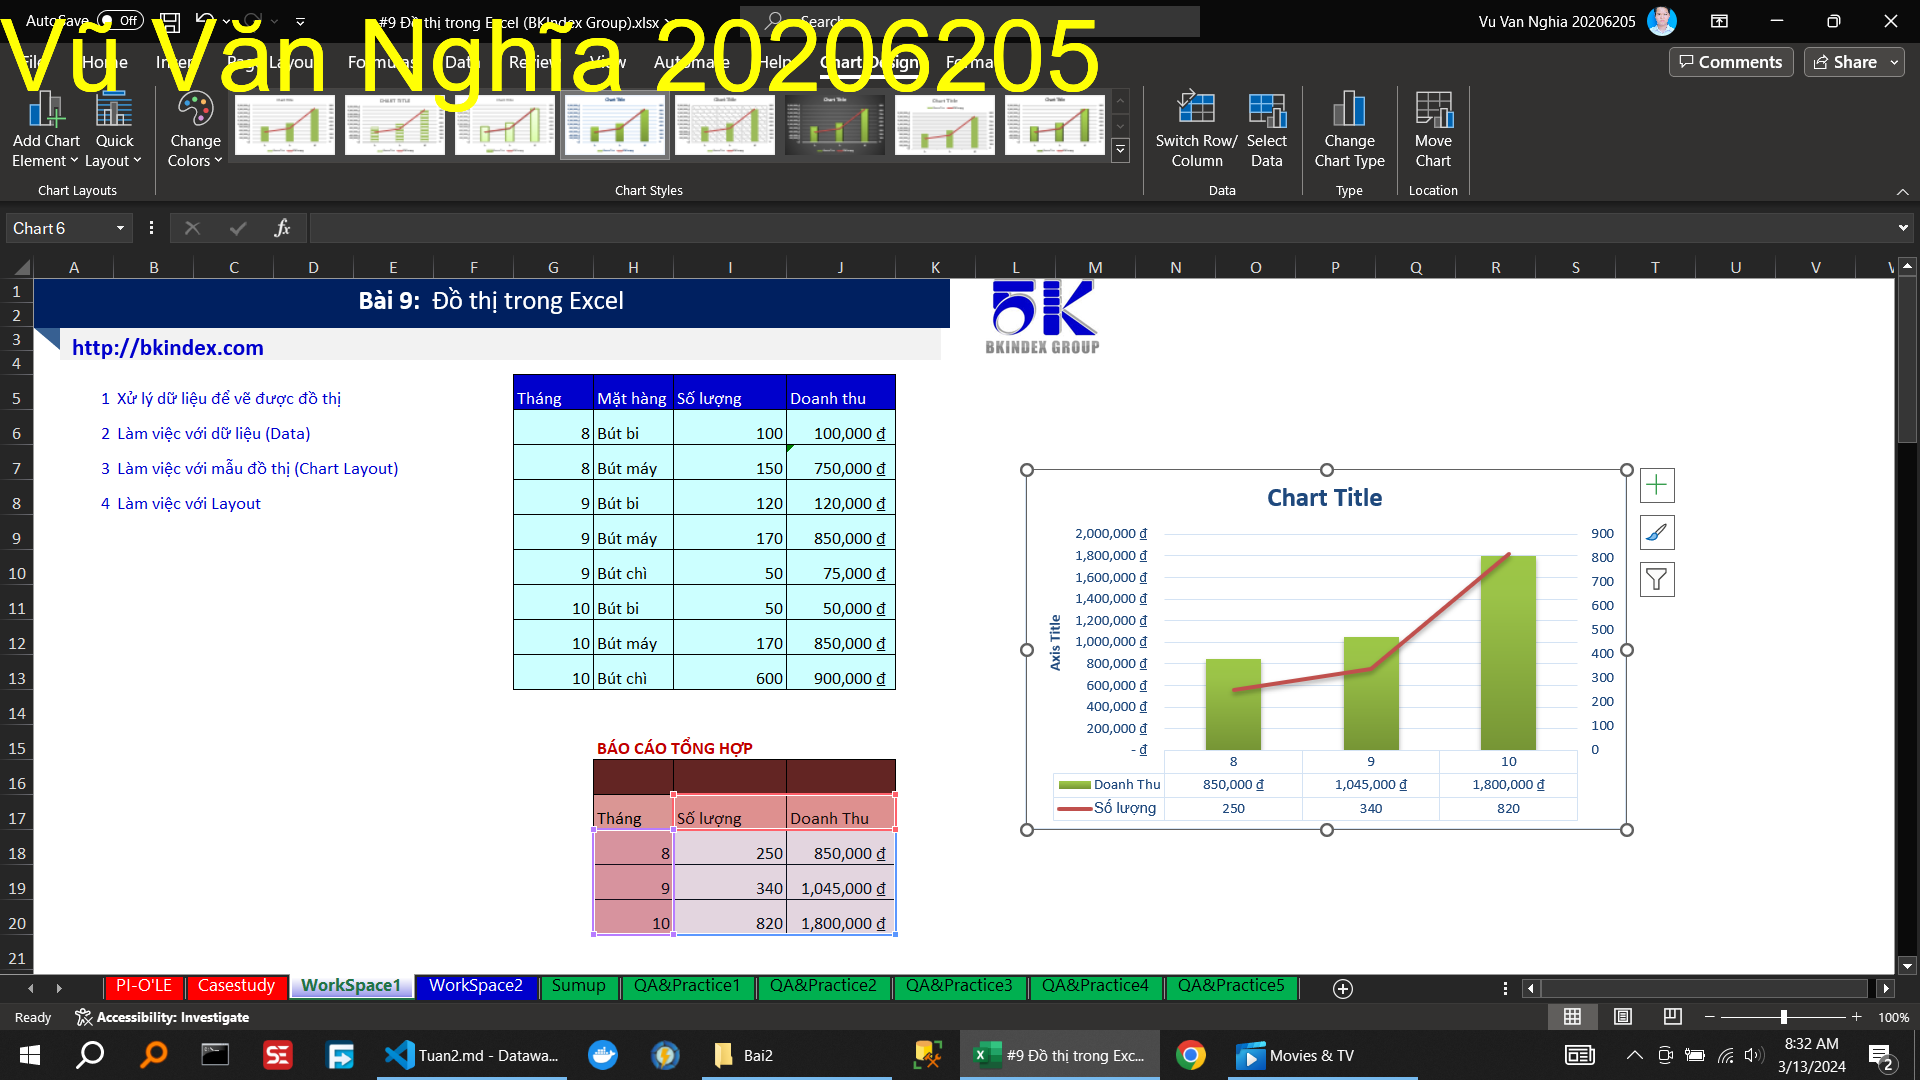
\includegraphics[scale = 0.15]{Bai2/HuongDan/2.png}
\caption{Hướng dẫn làm việc với mẫu đồ thị (Chart Layout)}
\end{figure}

\begin{figure}[H]
\centering
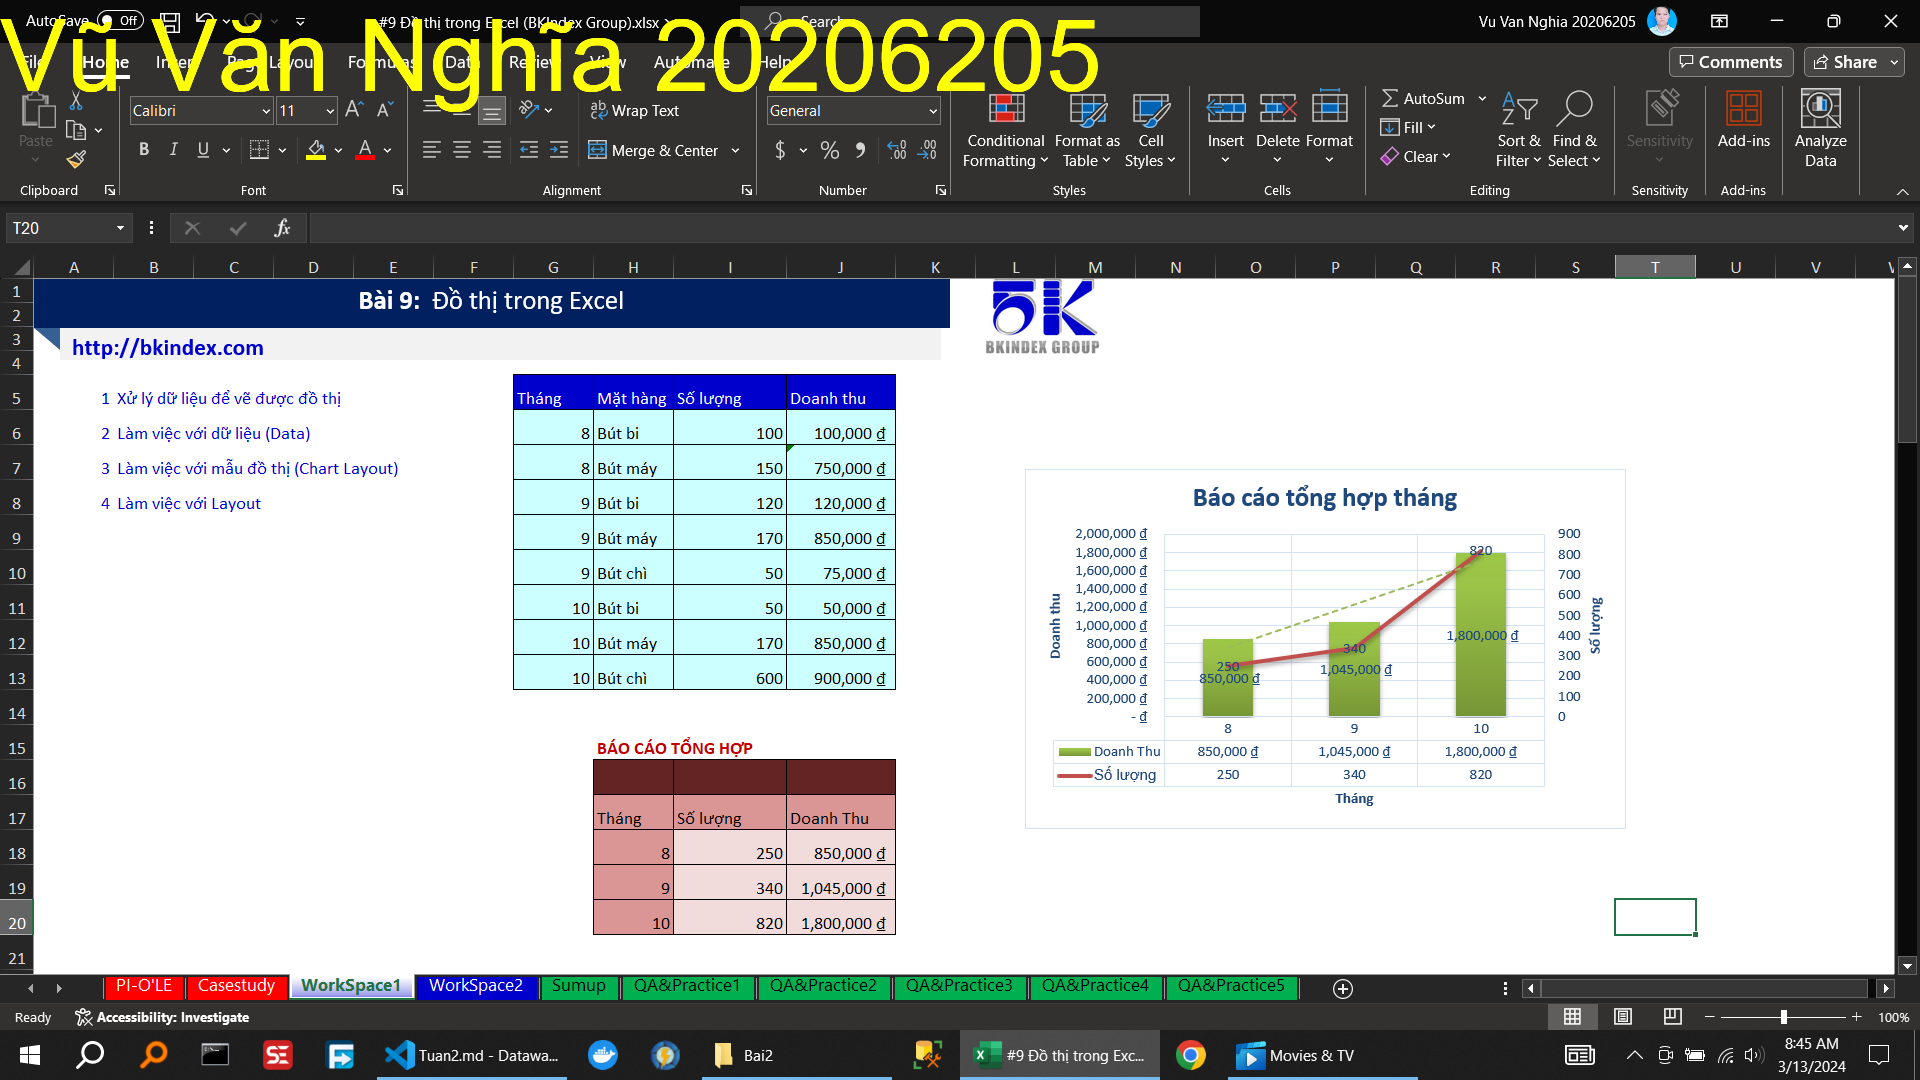
\includegraphics[scale = 0.15]{Bai2/HuongDan/3.png}
\caption{Hướng dẫn làm việc với Layout}
\end{figure}

\begin{figure}[H]
\centering
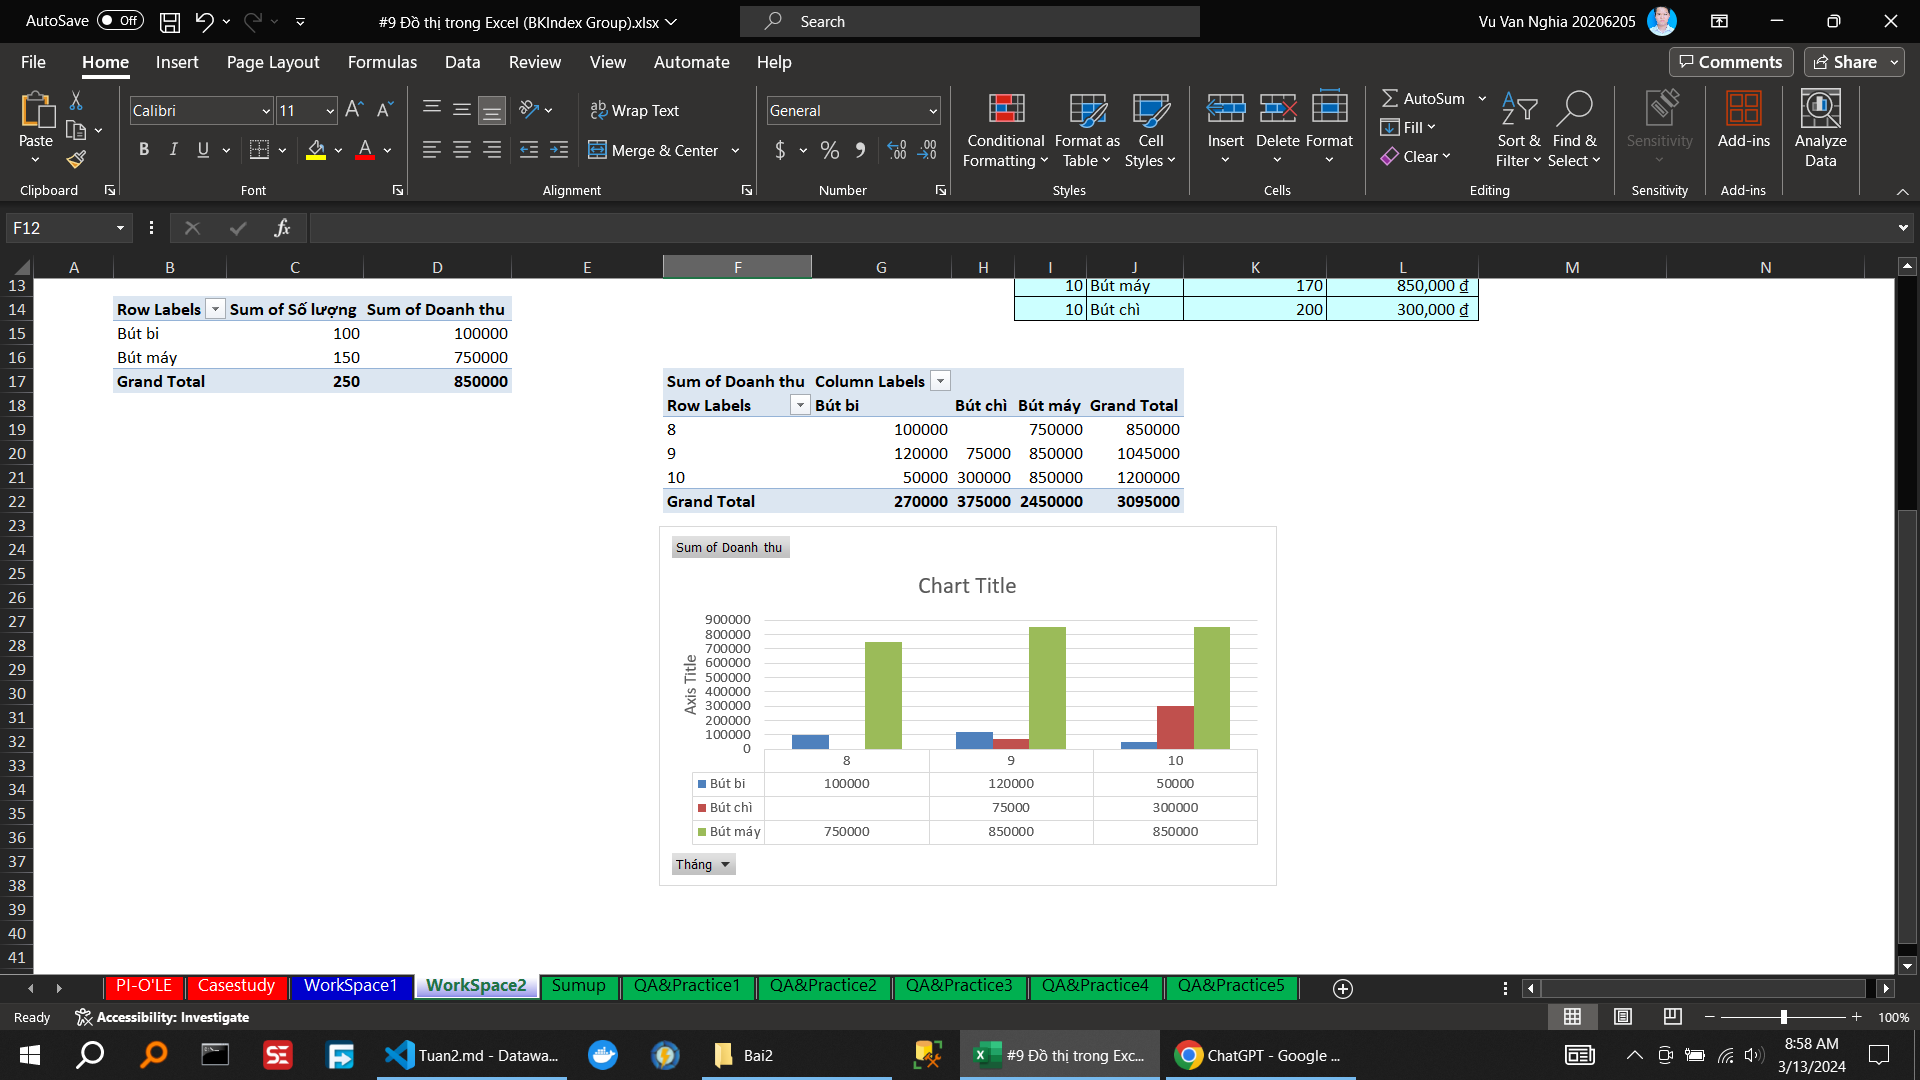
\includegraphics[scale = 0.15]{Bai2/HuongDan/4.png}
\caption{Hướng dẫn làm đồ thị trong 60s (với Pilot Table)}
\end{figure}

\begin{figure}[H]
\centering
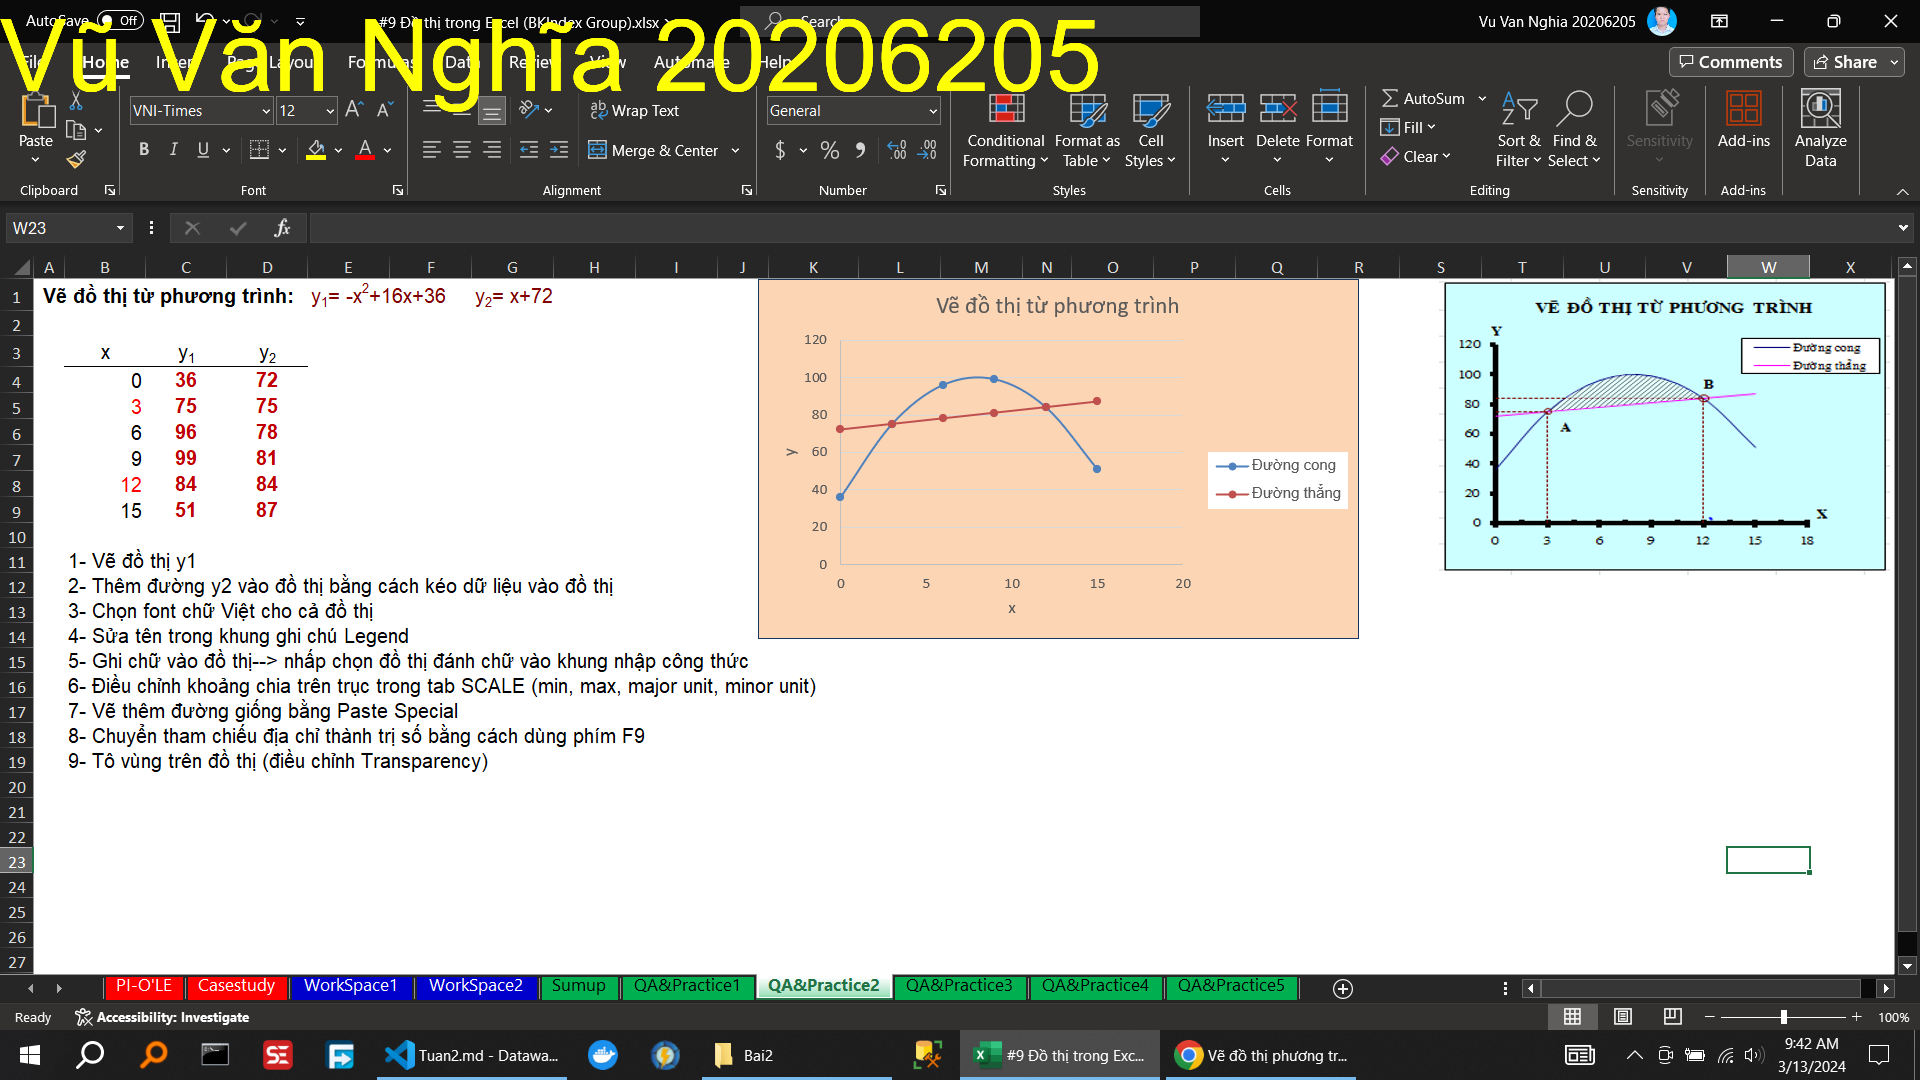
\includegraphics[scale = 0.15]{Bai2/ThucHanh/0.png}
\caption{Thực hành vẽ đồ thị giao nhau}
\end{figure}

\begin{figure}[H]
\centering
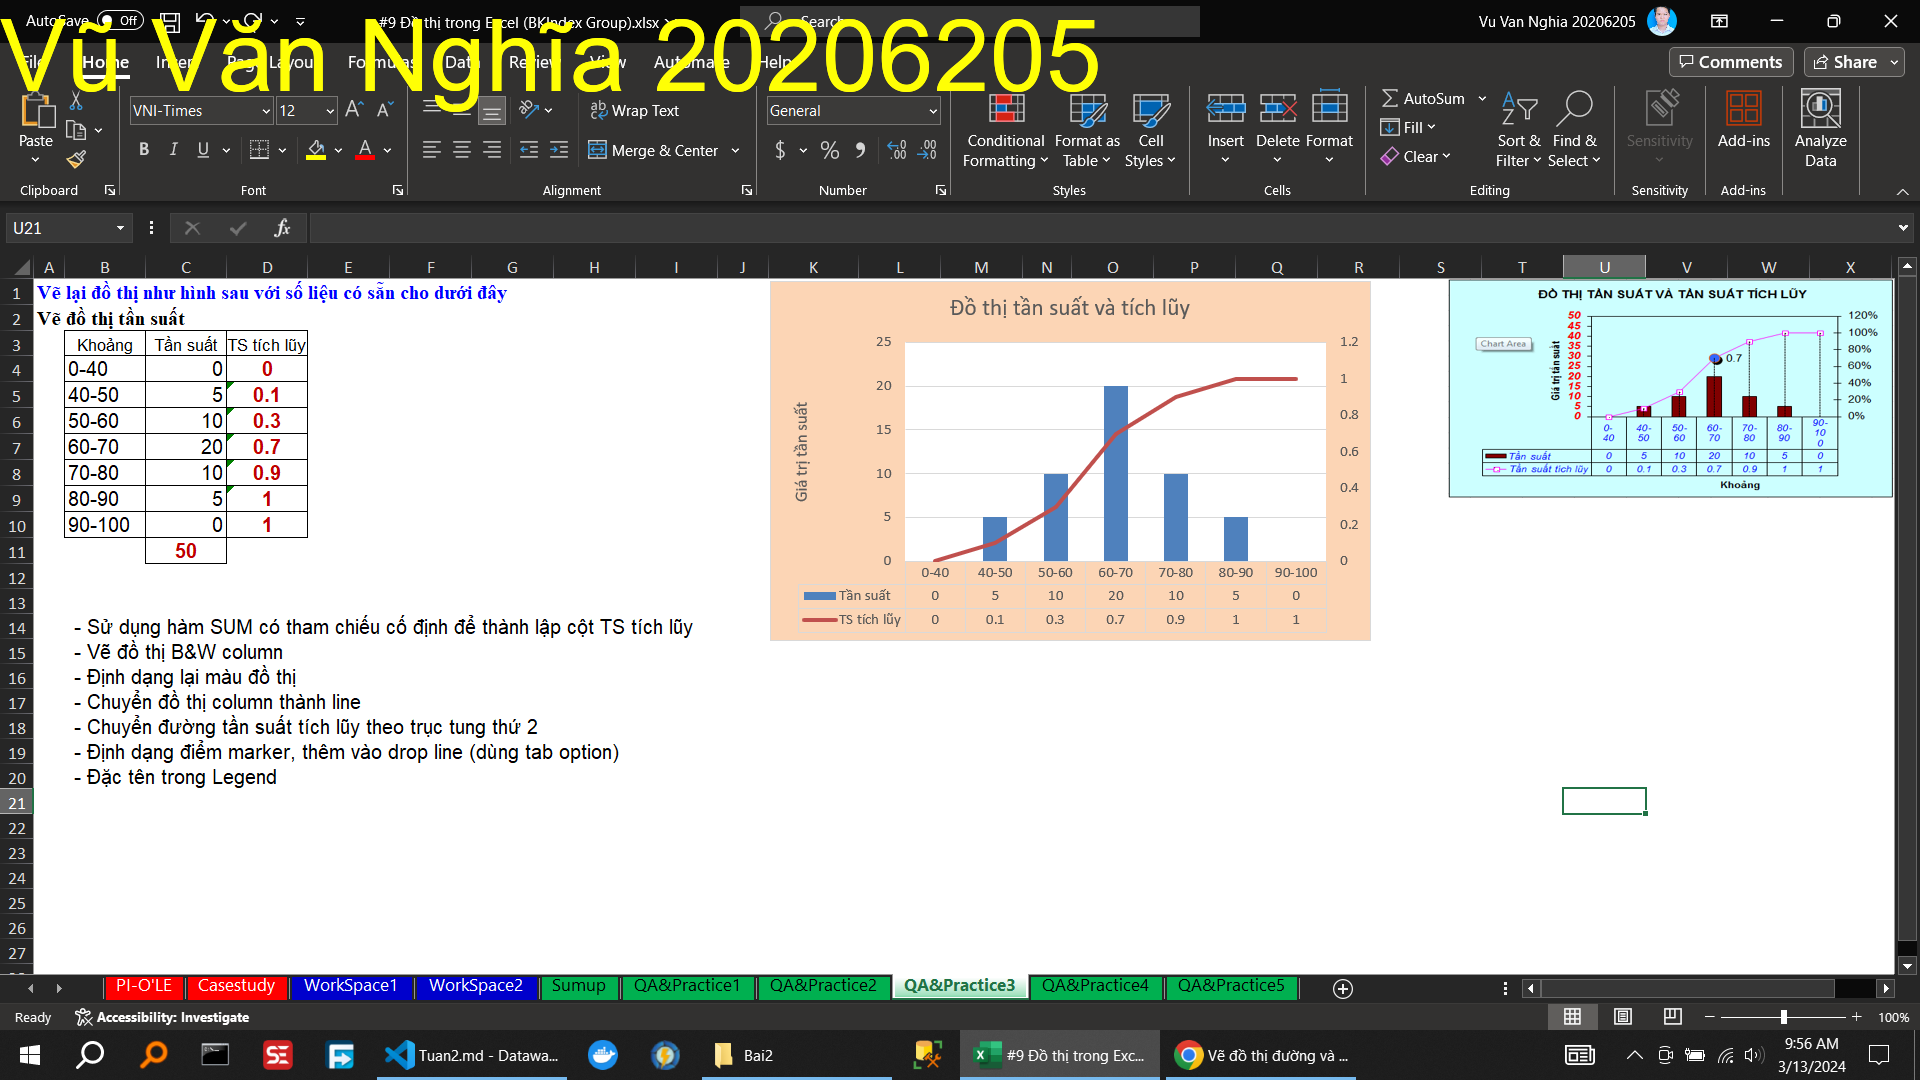
\includegraphics[scale = 0.15]{Bai2/ThucHanh/1.png}
\caption{Thực hành vẽ đồ thị tần suất và tích lũy}
\end{figure}

\begin{figure}[H]
\centering
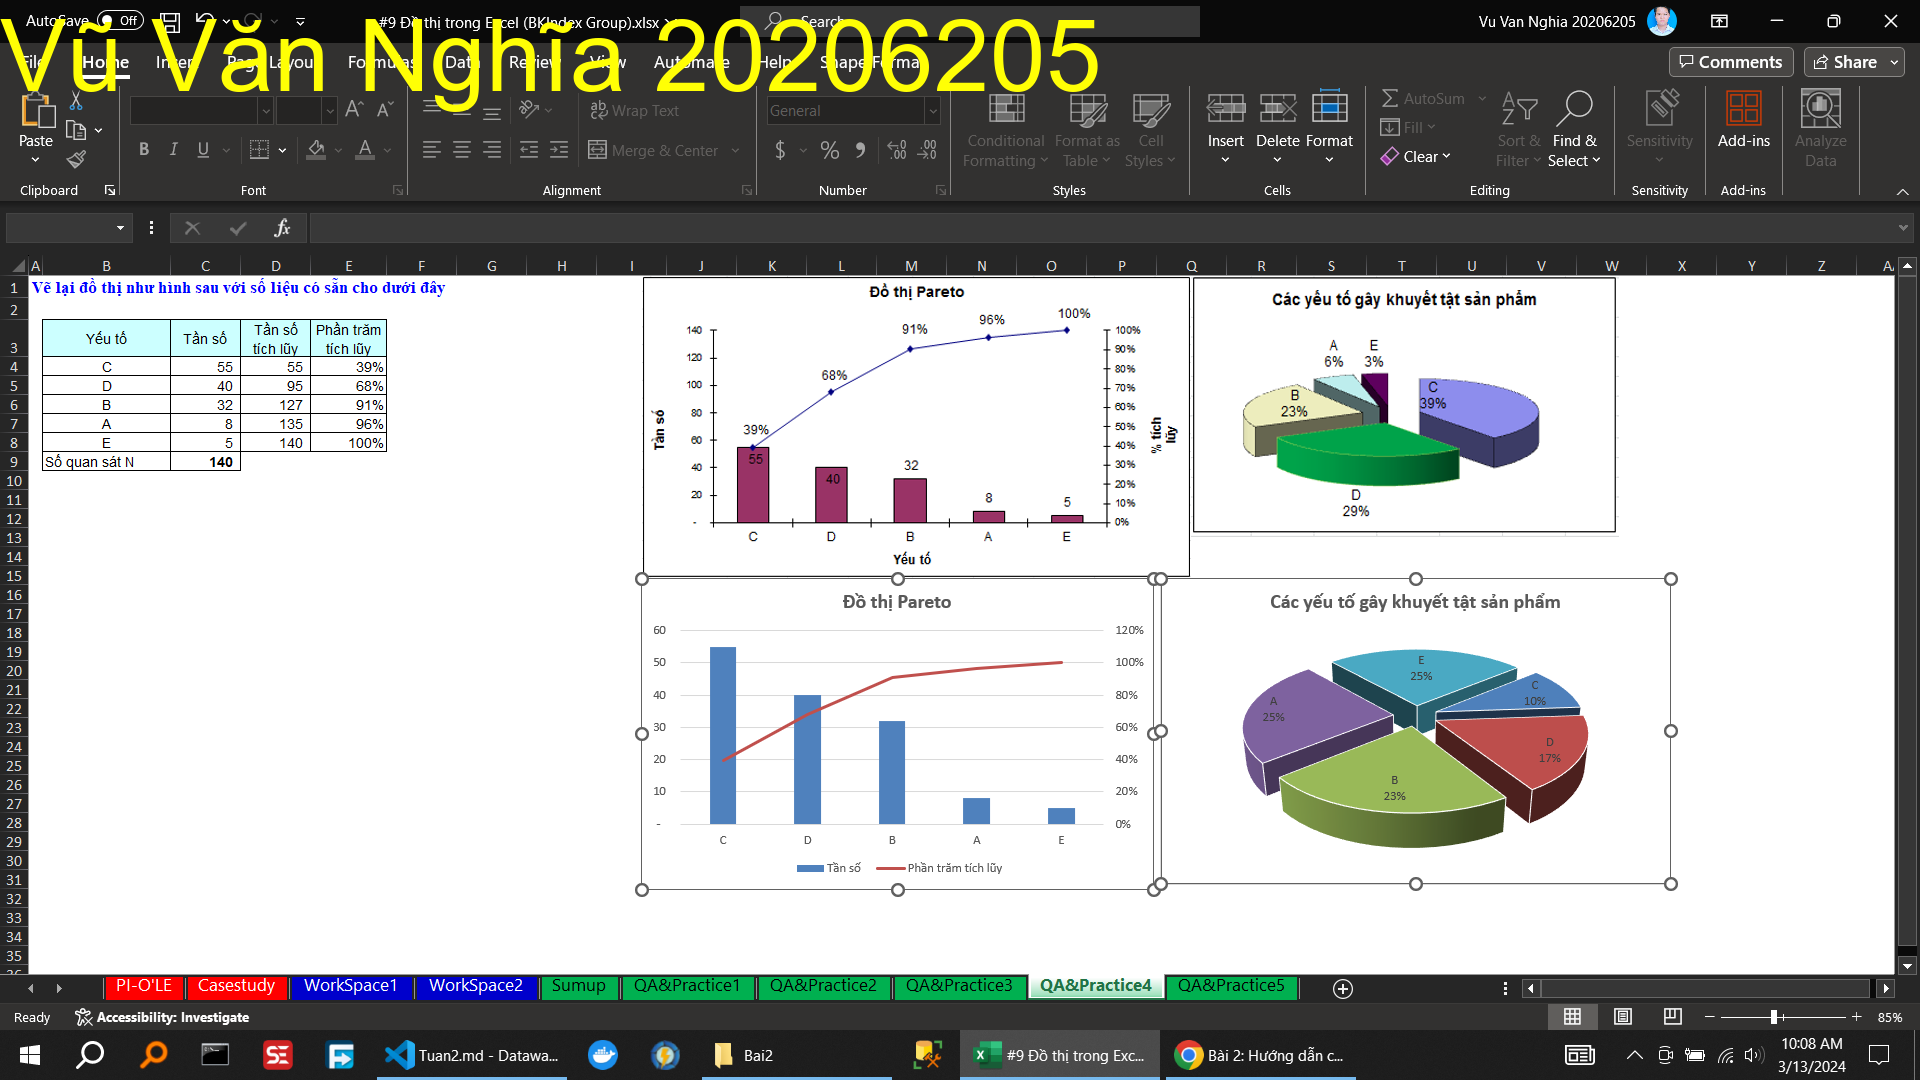
\includegraphics[scale = 0.15]{Bai2/ThucHanh/2.png}
\caption{Thực hành vẽ đồ thị hình bánh}
\end{figure}

\begin{figure}[H]
\centering
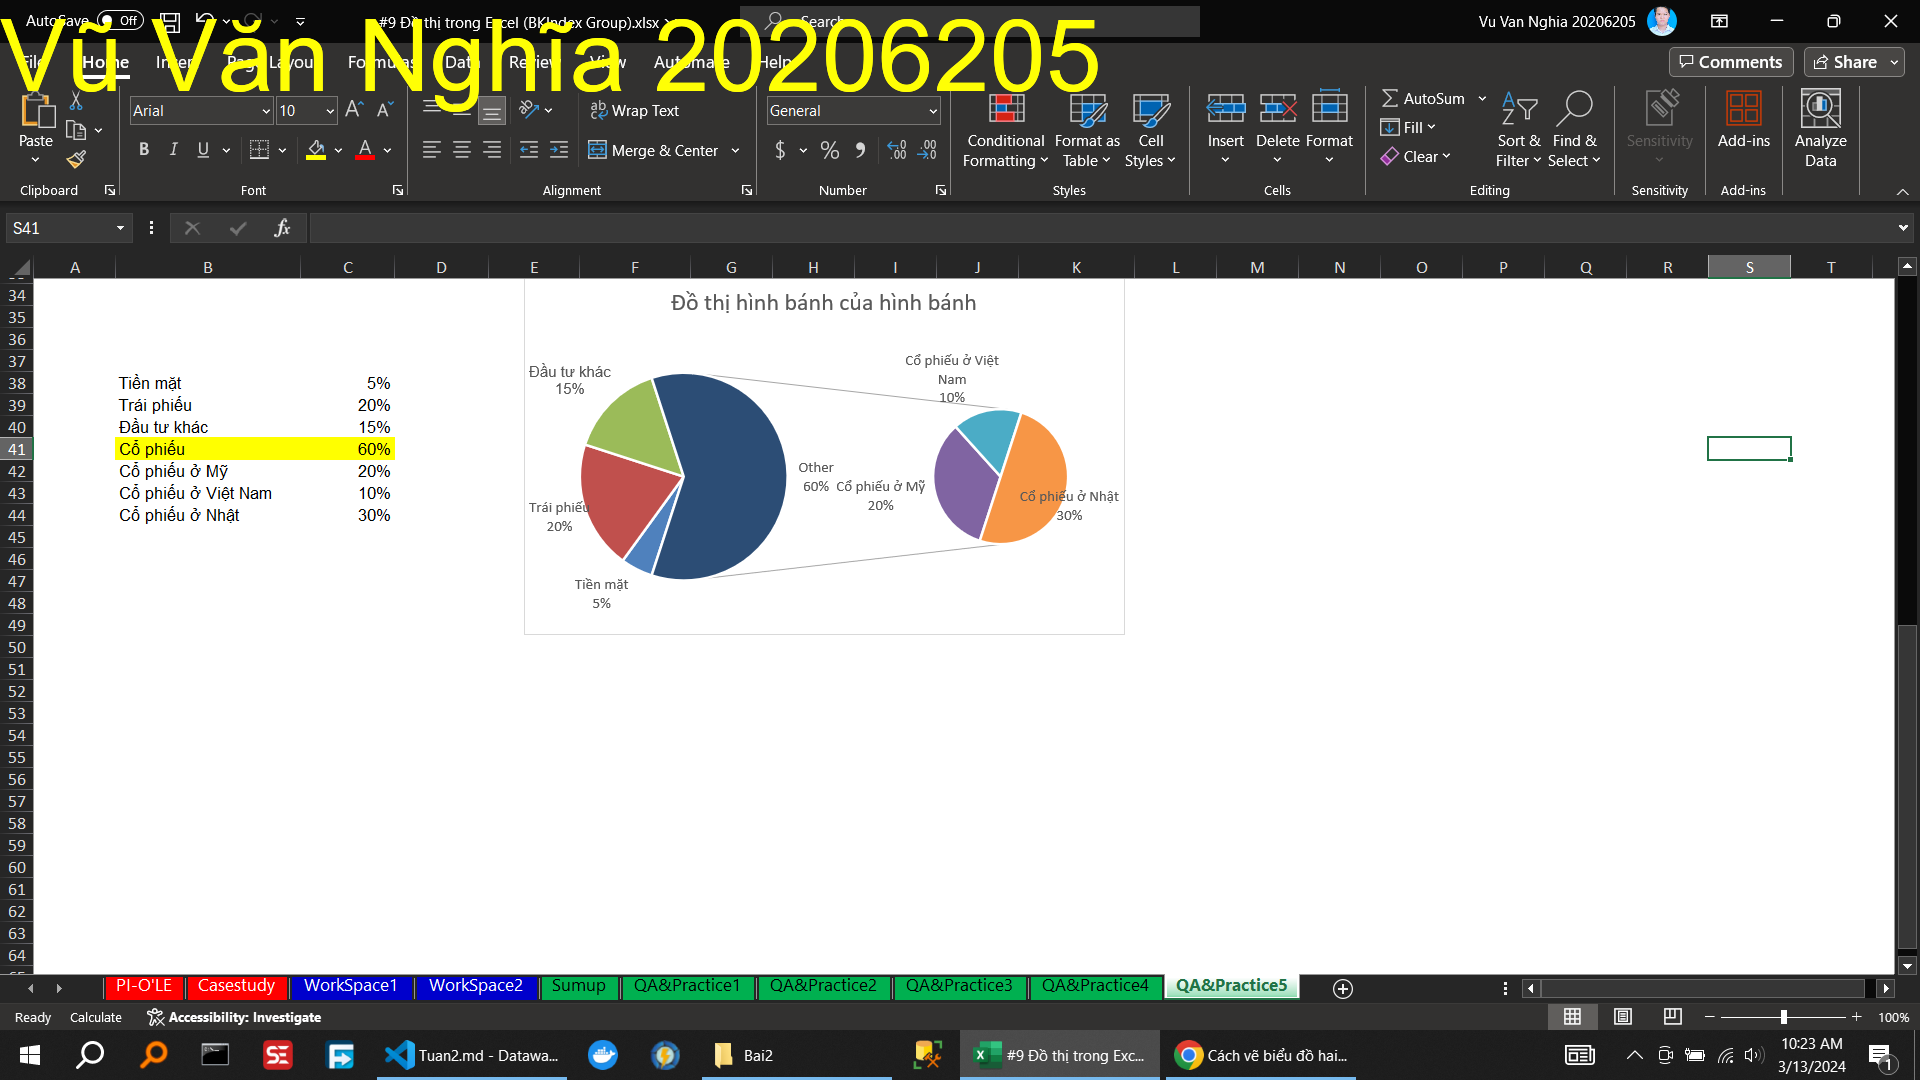
\includegraphics[scale = 0.15]{Bai2/ThucHanh/3.png}
\caption{Thực hành vẽ đồ thị hình bánh của hình bánh}
\end{figure}

%%%%%%%%%%%%%%%%%%%%%%%%%%%%%%%%%%%%%%%%%%%%%%%%%%%%%%%
\subsection{Bài 3}

%%%%%%%%%%%%%%%%%%%%%%%%%%%%%%%%%%%%%%%%%%%%%%%%%%%%%%%
\end{document}
%%%%%%%%%%%%%%%%%%%%%%%%%%%%%%%%%%%%%%%%%%%%%%%%%%%%%%%